%\documentclass{beamer}
\documentclass[a4paper,9pt]{beamer}
\usepackage{colortbl}
%\documentclass{12pt}
\usepackage{graphicx}
\usepackage{epsfig}
\usepackage[english]{babel}
\usepackage{beamerthemesplit} % new
\usepackage{amsmath}
\usepackage{amssymb}
\usepackage{latexsym}
%\usetheme[showpagenr=tue]
%\newcounter{saveenumi}
%\newcounter{saveenumii}
%\newcounter{saveenumiii}
%\insertframnumber
%\inserttotalframenumber
%\usepackage[latin1]{inputenc}
% or whatever
\mode<presentation>
{
 \usetheme{Frankfurt}
 \usecolortheme{rose}
  \setbeamercovered{transparent}
}


\usepackage{times}
\usepackage[T1]{fontenc}
%\usepackage{fontenc}
%\usepackage{fourier}

%%%%%%%%%%%%%%%%%%%%%%%%%%%%%%%%%%%%%%%%%%%%%%%%%%
\title{eTourPlan: A Knowledge-Based\\ Tourist Route and Activity Planner}
\subtitle{Thesis Oral Defence for MCS Degree Program}
\author{Tshering Dema}
\institute{\normalsize Faculty of Computer Science\\
\vspace{0.1in}
\Large University of New Brunswick}

\begin{document}
\begin{frame}
  \titlepage
\end{frame}


\frame{\frametitle{Acknowledgement}
\begin{itemize}
%\begin{columns}[c] % the "c" option specifies center vertical alignment
%\column{.5\textwidth} % column designated by a command
\color{blue}\item Supervisors: \vspace*{0.1cm} 
\begin{itemize}
\item Dr. Harold Boley
\item Dr. Przemyslaw Rafal Pochec
\end{itemize}
\vspace*{0.2cm} 
%\item Problems \vspace*{0.3cm} 
%\item Objectives \vspace*{0.3cm} 
\color{blue}\item Committee members: \vspace*{0.1cm} 
\begin{itemize}
\item Dr. Bruce Spencer  
\item Dr. Gerhard Dueck
\item Dr. Yevgen Biletskiy
\end{itemize} 
\vspace*{0.2cm} 
%\item Testbed Architecture \vspace*{0.3cm} 
%\column{.5\textwidth}
%\item Testbed Architecture \vspace*{0.3cm} 
\color{blue} \item The Bhutan Project funded by Canadian International Development Agency (CIDA)\vspace*{0.2cm} 
\color{blue} \item University of New Brunswick (UNB) \vspace*{0.2cm} %\item References \vspace*{0.3cm} 
%\end{columns}
\end{itemize}
}


\frame{\frametitle{Outline}
\begin{enumerate}
%\begin{columns}[c] % the "c" option specifies center vertical alignment
%\column{.5\textwidth} % column designated by a command
\item Introduction \vspace*{0.3cm} 
%\item Problems \vspace*{0.3cm} 
%\item Objectives \vspace*{0.3cm} 
\item Background \vspace*{0.3cm} 
%\item Testbed Architecture \vspace*{0.3cm} 
%\column{.5\textwidth}
%\item Testbed Architecture \vspace*{0.3cm} 
\item Knowledge Base Design: Ontology and Facts \vspace*{0.3cm} 
\item Knowledge Base Design: Rules \vspace*{0.3cm} 
\item Evaluation of eTourPlan on the Bhutan KB \vspace*{0.3cm} 
\item Conclusion and Future Work \vspace*{0.3cm} 
%\item References \vspace*{0.3cm} 
%\end{columns}

\end{enumerate}
}

%%%%%%%%%%%%%%%%%%%%%%%%%%%%%%%%%%%%%%%%%%%%%%%%%%
%slide 2
\section{1. Introduction}

\subsection{1.1 Overview}
\frame{\frametitle{1.1 Introduction}
 \vspace{0.2in}
\centering {\Large \color{blue}\textbf{A knowledge-based eTourism prototype}}
 \vspace{0.25cm}
\begin{figure}[h] 
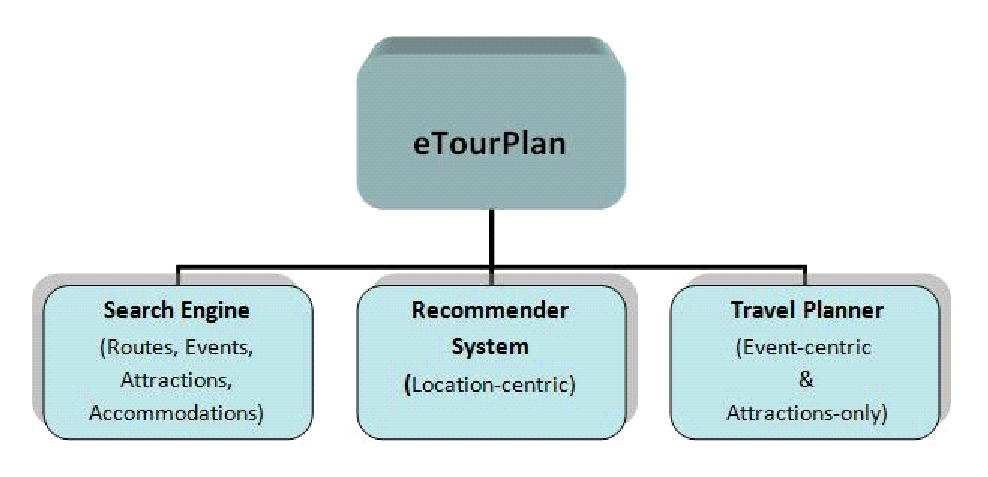
\includegraphics[width=10cm, height=5.5cm]{eTourPlan}
\end{figure}%\item Parametric search of tourist entities
%\item Recommend touristic route
%\item Recommmend activities for user-preferred provinces
%\item Plan an attraction or event-centric travel
}
\subsection{1.2 Motivation}
\frame{\frametitle{1.2.1 Motivation}
\begin{itemize}
\item Tourism is the world's largest and fastest growing industry
\vspace{0.2cm}
\item The World Tourism Organization predicts that one billion international tourists will travel by the year 2010
\vspace{0.2cm}
\pause
\item Most of the prevalent travel recommenders are location-centric\\
\begin{itemize}
 \item {\color{red}Shortcoming}: Do not function as complete trip planners. \\e.g., time (visit a number of places) > time (available to traveller)
\end{itemize}
\pause
\vspace{0.2cm}
\item Pre-customized travel packages in mass tourism
\begin{itemize}
 \item {\color{red}Shortcoming}: limited flexibility to users' preference specification
\end{itemize}
\vspace{0.2cm}
\pause
\item Independent sources for various tourist facility information \\(activity and accommodation)
\begin{itemize}
 \item {\color{red}Shortcoming}: Tourist consultants and travellers must visit multiple independent sources to plan a trip tailored to given preferences
\end{itemize}
\end{itemize}
}

\subsection{1.2 Motivation}
\frame{\frametitle{1.2.2 Motivation}
\begin{itemize}
\item {\color{blue}eTourism} is an information-based heterogenous business (distributed nature of its high volume of information)
\vspace{0.2cm}
 \begin{itemize}
 \item Information gathering, integration, distribution, and exchange are the backbones of the travel industry
\end{itemize}
\vspace{0.3cm}
\item  {\color{blue}The Semantic Web} is a major endeavour to enhance the Web by enriching its content with semantic (meta)data that can be processed by inference-enabled Web applications
\vspace{0.2cm}
 \begin{itemize}
 \item Modelling a well-structured and comprehensive Knowledge Base (KB) for consulting will help bolster the eTourism domain
\end{itemize}
\end{itemize}
}


%%%%%%%%%%%%%%%%%%%%%%%%%%%%%%%%%%%%%%%%%%%%%%%%%
\subsection{1.3 Objectives}
\frame{\frametitle{1.3 Objectives}
\textbf{\color{blue}To design, implement, and evaluate a knowledge-based eTourism prototype for Bhutan} 
\vspace{0.2cm}
\pause
\begin{itemize}
\item To design a light-weight ontology %using the Resource Description Framework Schema (RDFS)
      to capture all the tourism subdomains [aligned with the \textbf{Harmonise} eTourism ontology]
\vspace{0.2cm}
\pause
\item To build a Bhutan fact base consisting of \textbf{FOAF-like} profiles for tourist entities, structured by this ontology %using the Object-Oriented Rule Markup Language (OO RuleML) in its presentation syntax of the Positional-Slotted Language (POSL). 
\vspace{0.2cm}
\pause
\item To implement rule subsystems needed for generating \textbf{travel plans} containing \textbf{tour recommendations}:
\begin{itemize}
\item Partonomy rules for the subdivision of regions
\item Derivation rules to deduce transitive closure facts about distances etc.
\item Inference rules for various planning and recommendation modes
\item Query rules to perform semantic searches
\end{itemize}
\vspace{0.2cm}
\pause
\item To evaluate the overall operation of the eTourPlan prototype as run in the \textbf{OO jDREW} reasoning engine prototype (giving feedback to the OO jDREW open source community)
\end{itemize}
}

\frame{\frametitle{1.4 Travel Planner}
\centering {\LARGE \color{blue}\textbf{eTourPlan}}
 \vspace{0.45cm}
\begin{itemize}
 \item A knowledge-based eTourism prototype using Semantic Web techniques:
\begin{itemize}
\item \vspace{0.2cm}A well-structured and comprehensive KB for tourism subdomains
\item \vspace{0.2cm}Rule subsystems for search, recommendation and travel planning
\item \vspace{0.2cm}Utilizing Bhutan tourist information as a use case
\item \vspace{0.2cm}Results of running eTourPlan in the prototype RuleML engine OO jDREW are reported
\vspace{0.3cm}
\end{itemize}
\end{itemize}
}

%\item To evaluate the KB by systematically testing each of the rule subsystems with varying user preferences.\vspace{0.3cm}

%%%%%%%%%%%%%%%%%%%%%%%%%%%%%%%%%%%%%%%%%%%%%%%%%%
\section{2. Background}
\subsection{2.1 Tour Planner and Recommender Systems}
\frame{\frametitle{2.1.1 Travel Planning Strategies}
\small
\raggedright
\begin{table}[tbph]
%\label{table:alarms}
\begin{tabular}{|l|l|l|l|}
\hline
       &$~~$Attraction-Only &$~~~~~$Event-Only &$~~~~~~$Event-Centric\\
       & $~~~~~~$Planning&$~~~~~~$ Planning&$~~~~~~~~$Planning\\
\hline
\rowcolor{yellow}
Complete & Planning attractions   & Planning events  & Planning events with  \\

\rowcolor{yellow}
Planning & based on related & based on their   & additional attraction \\

\rowcolor{yellow}
         &locations & dates and locations        & recommendation\\
       
\hline
Sequence& System orders the &  System orders the    & System orders both  \\
Planning& user-specified attra- &user-specified events &events and attractions \\
       &   ctions & & \\
\hline 
Partial& System orders and &  System orders and     & System orders and  \\
Planning&adds to user-specified &adds to user's             &adds to user's \\
        &attractions &specified events  &specified events and \\
        &           &          &attractions  \\  
                 
\hline      
\end{tabular}
 % \end{minipage}
  %\begin{minipage}{5.0cm}
  %\caption{ER eth2}
    %\end{minipage}
%\caption{packet loss for each rate and burst}
\end{table}
}

%%%%%%%%%%%%%%%%%%%%%%%%%%%%%%%%%%%%%%%%%%%%%%%%%%%
\frame{\frametitle{2.1.2 Recommender System}
%\color {blue} Prevalent recommender systems: \\(like Triplehop's TripMatcher and Me-Print used by Travelocity) 
%\begin{itemize}
%\item Do not support complete user-defined trip package
%\end{itemize}
%\vspace{0.3cm}
\textbf{Knowledge-based Recommenders}
\begin{itemize}
\item Use ontologies and rules for knowledge representation
\item Derive implicit facts from ontology-structured facts using rules
\item Provide recommendations as wide-ranging as its KB
\item Respond to user's stated requirements
\vspace{0.3cm}
\end{itemize}
\color {red} \large \textbf{A ``NEED" for providing trip planning options}
%However,it is tedious to support multiple decision styles and offer maximum options to users by a recommender system alone.\\
%Literature study supports the need of providing trip planning options along with recommendations to the travellers.
%\\Thus, building an integrated system of search engine, recommender, and planner.
}

\subsection{2.2 The Semantic Web}
\frame{\frametitle{2.2 The Semantic Web}
\textbf{\color{blue}Concept}
\begin{itemize}
\item Machine-understandable metadata
\item Knowledge representation and automatic data integration
\item Desirable for structuring vast information-based business (e.g. Tourism)
\end{itemize}
\vspace{0.3cm}
\textbf{\color{blue}Semantic Web techniques}
\begin{itemize}
\item Knowledge representation by using XML, RDF and ontologies
\item To perform inferences and automated reasoning using Description-Logic and/or Rule Engines 
\end{itemize}
}

\subsection{2.3 FOAF: Friend Of A Friend}
\frame{\frametitle{2.3 FOAF: Friend Of A Friend}
\textbf{\color{blue}Friend Of A Friend: Semantic Social Networking}
\begin{itemize}
\item Provides extended RDF Schema (RDFS) vocabulary
\item Person-centric RDF knowledge representation
\item Enables Semantic Web methods for formalised personal homepages
\end{itemize}
\vspace{0.3cm}
\color{blue} An approach similar to FOAF is transferred to semantically describe and link profiles for tourist entities
}


\subsection{2.4 The Harmonise Ontology}
\frame{\frametitle{2.4 The Harmonise ontology}
\textbf{\color{blue}Ontology:} Shared understanding of the relevant concepts and relationships of a domain\\
\vspace{0.3cm}
\textbf{\color{blue}Harmonise ontology:}
\begin{itemize}
\item eTourism ontology for information exchange in travel and tourism
\item Classifications of data items for events, attractions, accommodations, and restaurants
\item A market validation by 12 pilot organizations (based across Europe) through the Harmo-TEN project
\vspace{0.3cm}
\item Some key players in the Tourism Harmonization Network are:
 \begin{itemize}
 \item the Open Travel Alliance (OTA)
 \item the World Tourism Organization (WTO)
 \item the Travel Technology Initiative (TTI)
 \item the International Federation for IT, Travel and Tourism (IFITT)
\end{itemize} 
\end{itemize}
}


\subsection{2.5 Semantic eTourism Prototype}
\frame{\frametitle{2.5 Semantic eTourism Prototype}
\textbf{\color{blue} Machine-readable representation of information in the form of:}\\
\vspace{0.3cm}
\textbf{\color{blue}Ontologies:}
\begin{itemize}
\item Good basis for reasoning and classification
\item Uniform definitions of tourism subdomains
\item Remove semantic ambiguity
\end{itemize}
\vspace{0.3cm}
\textbf{\color{blue}Facts:}
\begin{itemize}
\item Object-centric descriptions of tourist entities
\end{itemize}
\vspace{0.3cm}
\textbf{\color{blue}Rules:}
\begin{itemize}
\item Semantic search against the above facts (formal knowledge) rather than keyword search 
      against texts (natural language)
\item Higher services based on deduction (Travel planning and recommendation)

\end{itemize}
}

%\subsection{2.5 Semantic eTourism Prototype}
%\frame{\frametitle{2.5 Tourism subdomains}
%\textbf{\color{blue}Five tourism subdomains defined by Encyclopedia of Tourism}
%\vspace{0.3cm}
%\begin{enumerate}
%\item\textbf{\color{blue}Regions}: Fundamental to partitioning the geography\\
%\begin{itemize}
%\item Helps in locating tourist entities
%\end{itemize}
%\vspace{0.3cm}
%\item \textbf{\color{blue}Transportation}: A vital role in the tourism infrastructure
%\begin{itemize}
%\item Connects tourist destinations
%\end{itemize}
%\vspace{0.3cm}
%\item \textbf{\color{blue}Accommodations}: Hotel, resort, guest\_house, etc
%\begin{itemize}
%\item Provides bedroom facilities on a commercial basis for tourists
%\end{itemize}
%\vspace{0.3cm}
%\item \textbf{\color{blue}Events}: One-time or periodic events
%\begin{itemize}
%\item Special soccer match, yearly cultural celebrations, Arts and entertainment, sports and education, etc
%\end{itemize}
%\vspace{0.3cm}
%\item \textbf{\color{blue}Attractions}: Places of interest open to public
%\begin{itemize}
%\item recreation, education or historical interest, etc
%\end{itemize}
%\end{enumerate}
%}

%\subsection{2.7 Rule Languages and Rule Engines}
%\frame{\frametitle{2.6 Rule Languages and Rule Engines}
%\begin{itemize}
%\item\textbf{\color{blue} Rule Markup Language (RuleML)}
%\begin{itemize}
%\item XML-based language for Web rules
%\item Permits both forward and backward rules
%\item Current version 0.91
%\item Object-Oriented RuleML 
%\end{itemize}
%\vspace{0.3cm}
%\item\textbf{\color{blue} Positional-Slotted Language (POSL)} 
%\begin{itemize}
%\item Derived from Prolog
%\item Presentation syntax for Semantic Web knowledge
%\item Compact Language
%\item POSL<->RuleML translator
%\end{itemize}
%\vspace{0.3cm}
%\item\textbf{\color{blue} OO jDREW: Object-Oriented Java Deductive Reasoning Engine for the Web}: 
%\vspace{0.3cm}
%\begin{itemize}
%\item OO jDREW BU (Bottom Up) execution -forward reasoning
%\item OO jDREW TD (Top Down) execution -backward reasoning
%\item OO jDREW Top-Down FindAll Solutions architecture
%\end{itemize}
%\end{itemize}
%}
%//////////////////////////////////////////////////////////////
\section{3. KB Design: Ontology and Facts}

\subsection{3.1 The eTourPlan Architecture}
\frame{\frametitle{3.1 The eTourPlan Architecture}
\begin{figure}[h] 
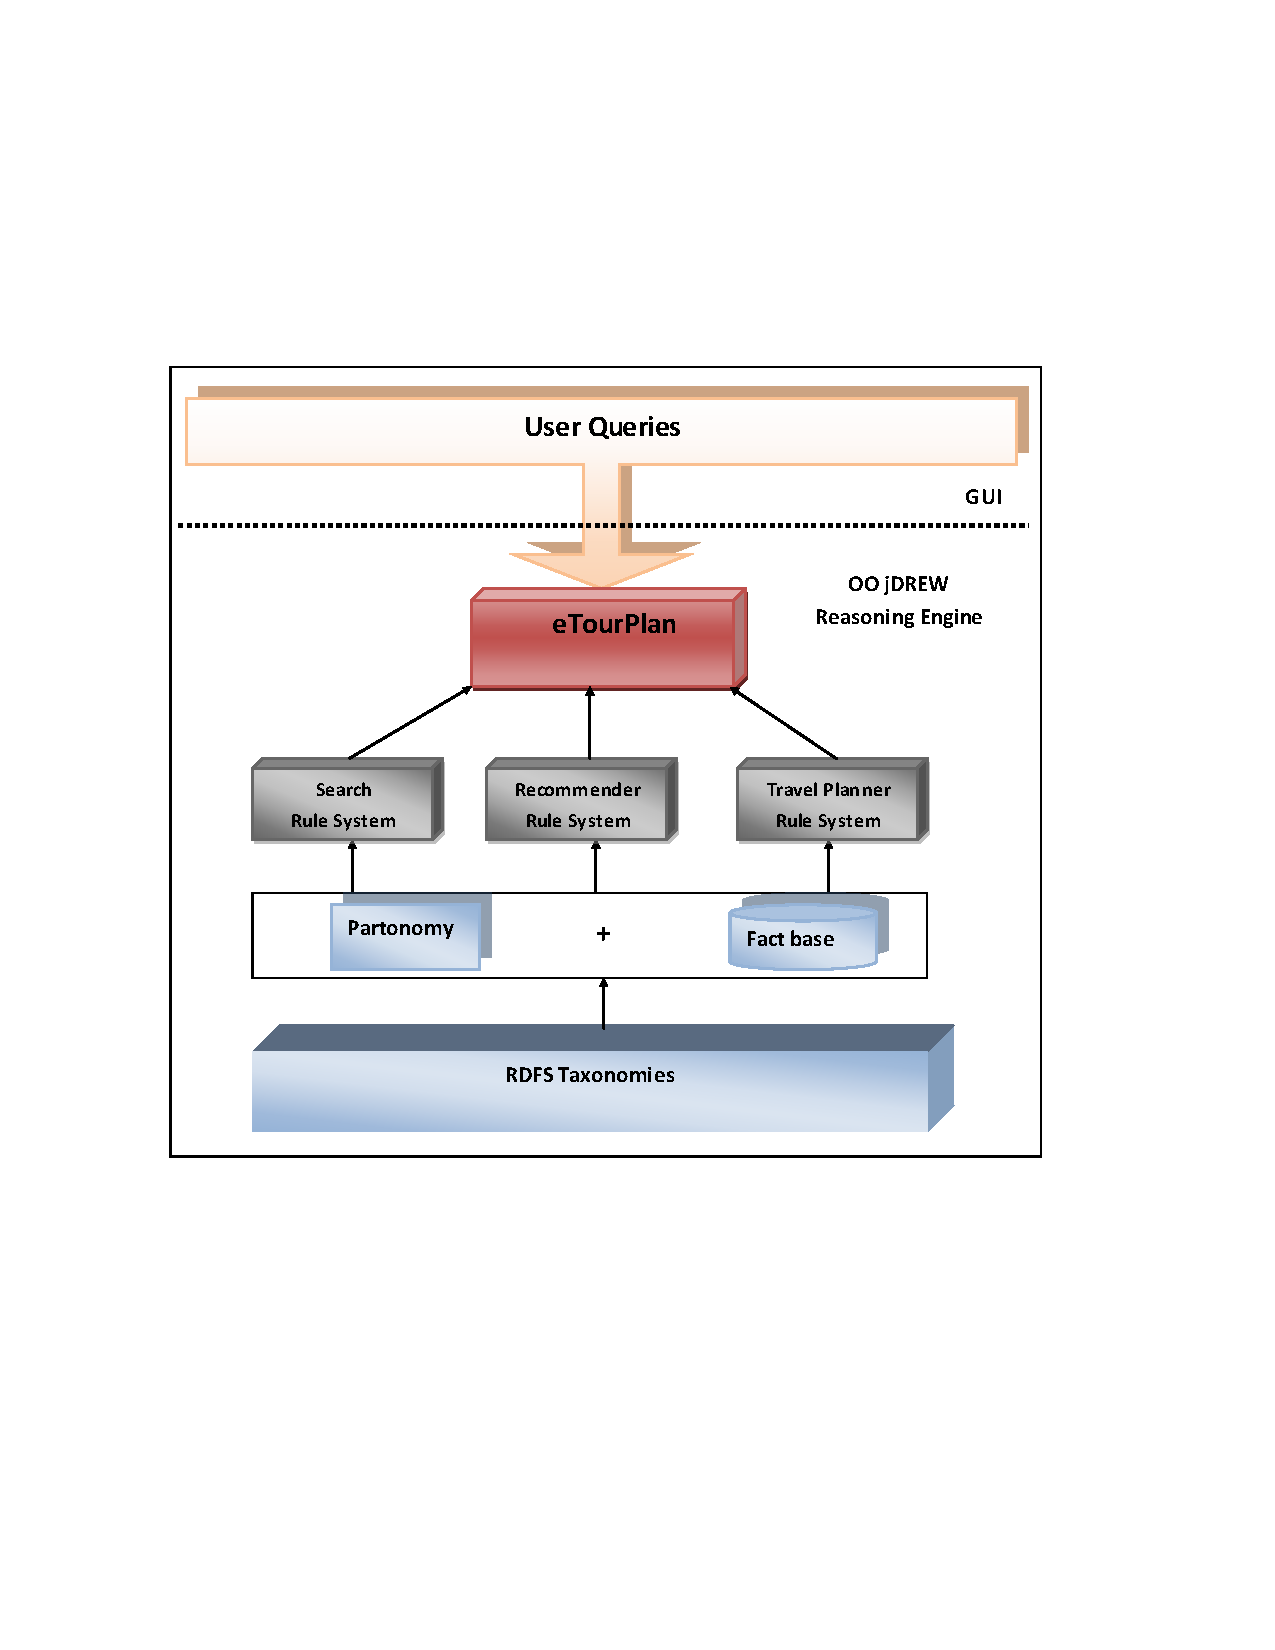
\includegraphics[width=10cm, height=7.5cm]{architecture.pdf}
\end{figure}
}

\subsection{3.2 Ontology Design}
\frame{\frametitle{3.2 Ontology Design}
 \begin{itemize}
 \item \vspace{0.2cm} `Reference model' for a specific domain
 \item \vspace{0.2cm} RDFS light-weight ontologies (adapted from the Harmonise eTourism ontology)
 \item \vspace{0.2cm} To stucture the FOAF-like profiles of tourist entities:
 \begin{itemize}
  \item province
  \item event
  \item attraction
  \item accommodation
 \end{itemize}
 \vspace{0.3cm}
 \item \textbf{\color{blue} Why Harmonise?}
 \begin{itemize}
 \item Mature and standard ontology
 \item Interoperability among many agents and applications
 \item Expressed in RDFS (SubClassOf hierarchies are supported by OO jDREW)
 \end{itemize}
 \end{itemize}
}

%%%%%%%%%%%%%%%%%%%%%%%%%%%%%%%%%%%%%%%%%%%%%%%%%%%%%%%%%%%%%%%%%%%%%%%%%%
\subsection{3.3 Ontology and FOAF-like Profile Descriptions of eTourPlan}
\frame{\frametitle{3.3.1 FOAF-like Province Profile}
\begin{figure} [tbph]
\centering
\begin{tabular}{|l|}
\hline
-----------------------------------------\\
\textbf{\color{blue}Profile of Thimphu Province}\\
-----------------------------------------\\
\textbf{province}({\color{red}Thimphu:Province}$^{\wedge}$\\
\hspace{0.5in}   {\color{blue}hs.url}->``{\color{red}http://www.thimphu.gov.bt}";\\
\hspace{0.5in}   {\color{blue}et.capital}->Thimphu\_City:City;\\
\hspace{0.5in}  {\color{blue}et.area}->``1,819 sq.km'';\\
\hspace{0.5in}   {\color{blue}et.elevation}-> ``1,300 to 7300 meters'';\\
\hspace{0.5in}   {\color{blue}et.numBlocks}->10:Integer;\\
\hspace{0.5in}   {\color{blue}et.numAttractions}->3:Integer;\\
\hspace{0.5in}   {\color{blue}et.numEvents}->2:Integer;\\
\hspace{0.5in}   {\color{blue}et.numAccommodations}->0:Integer;\\
\hspace{0.5in}    {\color{blue}hs.languagesSpoken}->``Dzongkha'';\\
\hspace{0.5in}    {\color{blue}hs.description}->``Thimphu is the capital of Bhutan'';\\
\hspace{0.5in}   {\textbf{\color{black} \large {hs.relatedTo}}}->{\color{red}Punakha:Province}).\\
\hline
\end{tabular}
\end{figure}
}

%%%%%%%%%%%%%%%%%%%%%%%%%%%%%%%%%%%%%%%%%%%%%%%%%%%%%%%%%%%%%%%%%%%%%%%%%%
\frame{\frametitle{3.3.2 Harmonise's {\color{red}``relatedTo"} relation between provinces in the KB}
\begin{figure}[h] 
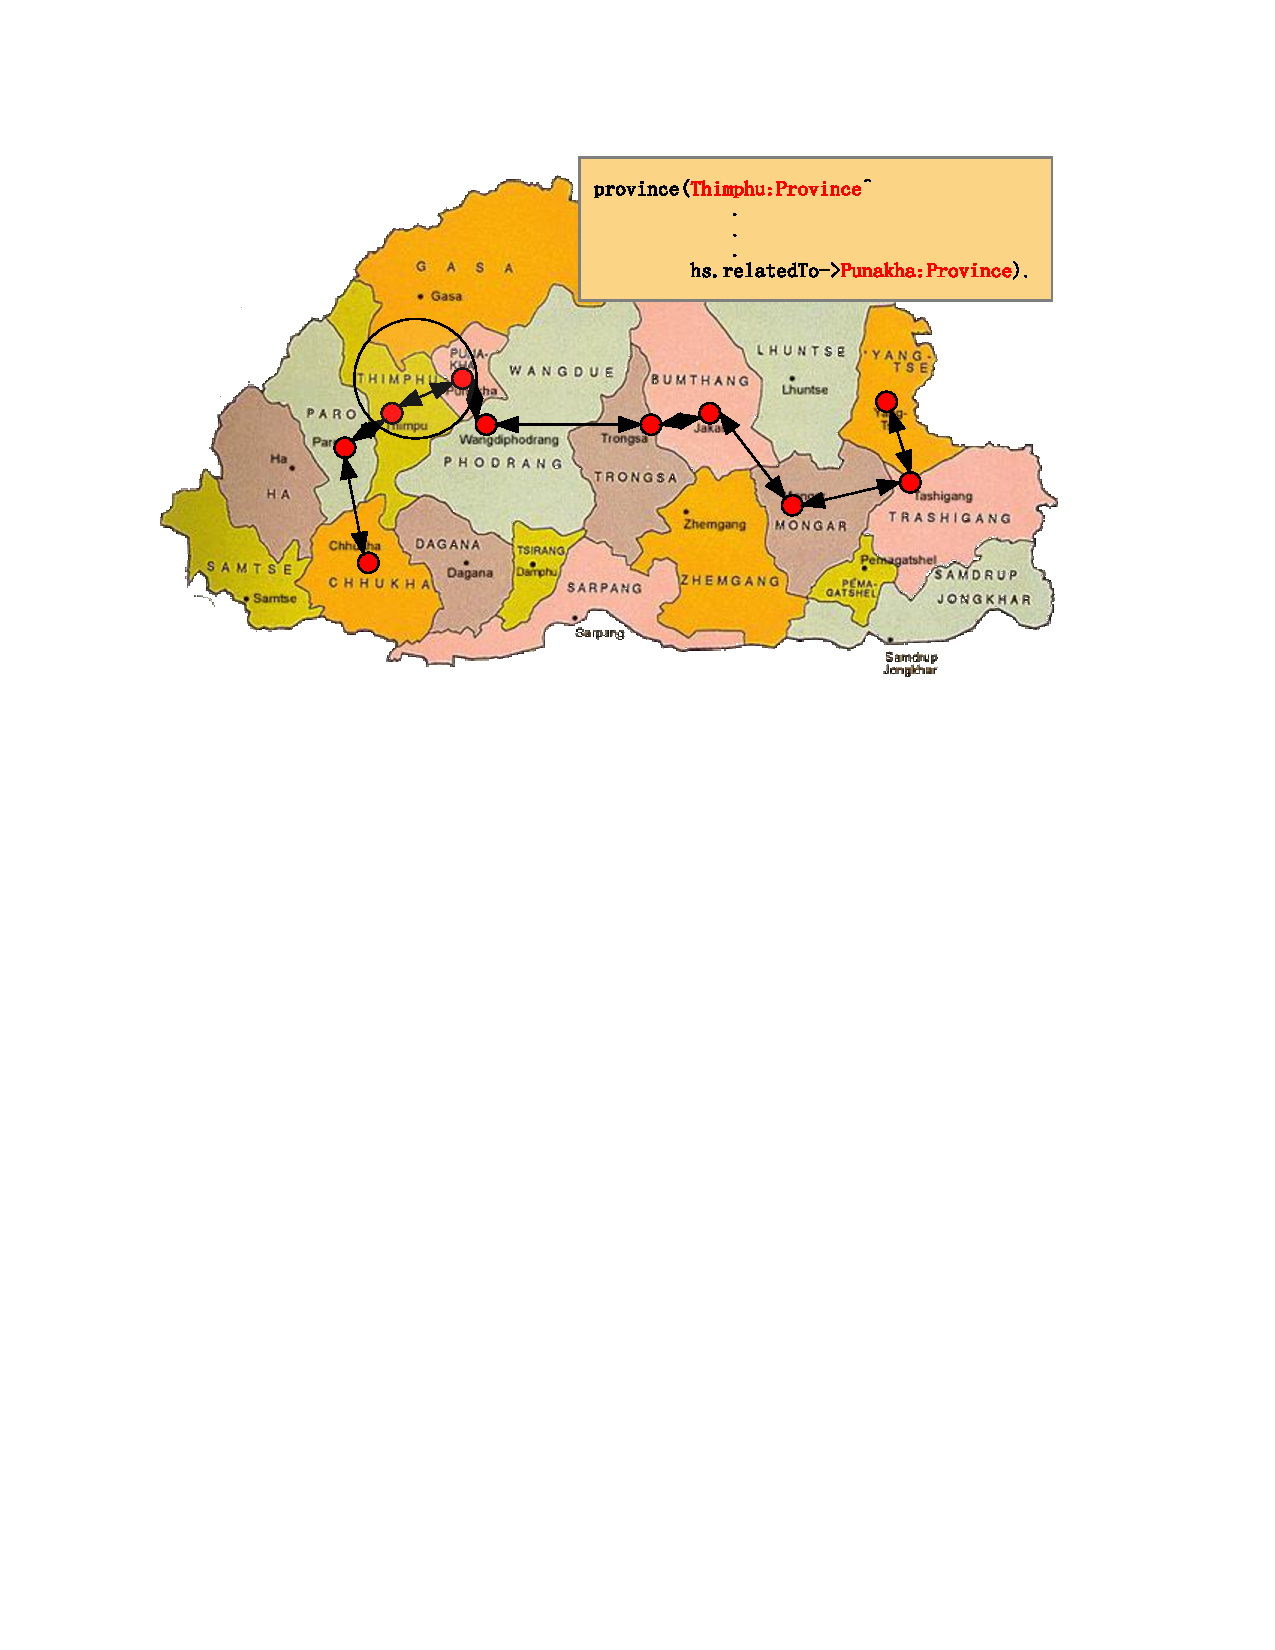
\includegraphics[width=10cm, height=6cm]{Provinces}
\end{figure}
}

%%%%%%%%%%%%%%%%%%%%%%%%%%%%%%%%%%%%%%%%%%%%%%%%%%%%%%%%%%%%%%%%%%%%%%%%%%
\frame{\frametitle{3.3.3 Events Class}
\begin{figure}[h] 
\includegraphics[width=10cm, height=6cm]{Events}
\end{figure}
}

%%%%%%%%%%%%%%%%%%%%%%%%%%%%%%%%%%%%%%%%%%%%%%%%%%%%%%%%%%%%%%%%%%%%%%%%%%
\frame{\frametitle{3.3.4 Attractions Class}
\begin{figure}[h] 
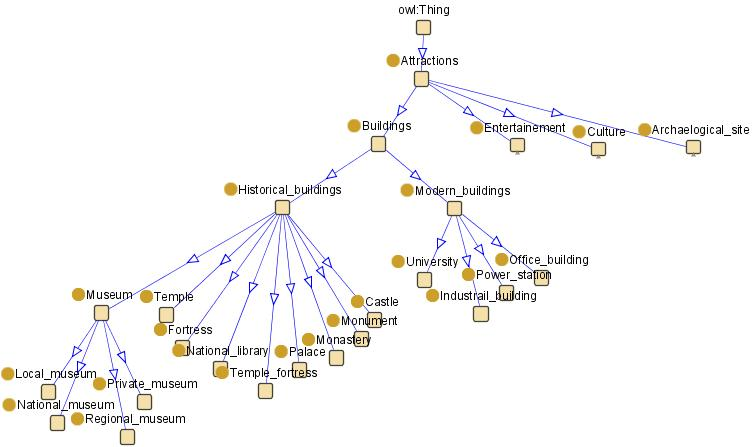
\includegraphics[width=10cm, height=6cm]{Attractions}
\end{figure}
}

%%%%%%%%%%%%%%%%%%%%%%%%%%%%%%%%%%%%%%%%%%%%%%%%%%%%%%%%%%%%%%%%%%%%%%%%%%

\frame{\frametitle{3.3.5 FOAF-like Profiles of an Event and an Attraction}
\begin{figure} [tbph]
\centering
\scriptsize
\begin{tabular}{|l|}
\hline
-----------------------------------------\\
\textbf{\color{blue}Profile of Thimphu\_Tshechu}\\
-----------------------------------------\\
\textbf{event}({\color{red}Thimphu\_Tshechu:Annual\_festival}$^{\wedge}$\\
   \hspace{0.35in}  {\color{blue}hs.url}->`` '';\\
   \hspace{0.35in}   {\color{blue} hs.startDate}->date[2008:Real,10:Real,09:Real];\\
   \hspace{0.35in}   {\color{blue} hs.endDate}->date[2008:Real,10:Real,11:Real];\\
   \hspace{0.35in}  {\color{blue} et.theme}->Cultural\_Religious\_Heritage;\\
   \hspace{0.35in}  {\color{blue} hs.location}->Tashichoe\_Dzong:Fortress;\\
   \hspace{0.35in}   {\color{blue} et.province}->Thimphu:Province;\\
   \hspace{0.35in}   {\color{blue} hs.description}->``It is a popular festival in Thimphu'';\\
   \hspace{0.35in}  {\color{blue}\textbf{\large{hs.relatedTo}}}->{\color{red}Thimphu\_Drupchen:Annual\_festival}).\\
\hline
\end{tabular}
\end{figure}
\begin{figure} [tbph]
\centering
\scriptsize
\begin{tabular}{|l|}
\hline
-----------------------------\\
\textbf{\color{blue}Profile of Ta\_Dzong}\\
-----------------------------\\
     \textbf{attraction}({\color{red}Ta\_Dzong:National\_museum}$^{\wedge}$\\
      \hspace{0.58in}   {\color{blue}hs.url}->``www.nationalmuseum.gov.bt/'';\\
      \hspace{0.58in}   {\color{blue}et.subblock}->Goepay:Village;\\
      \hspace{0.58in}   {\color{blue}et.province}->Paro:Province;\\
      \hspace{0.58in}   {\color{blue}et.theme}->Cultural\_Religious\_Heritage;\\
      \hspace{0.58in}   {\color{blue}et.open}->Open[DaysOfWeek[Tue, Wed, Thu, Fri, Sat, Sun],\\
       \hspace{1.45in}                            Period[10:Real, 16:Real]];\\
      \hspace{0.58in}   {\color{blue}et.capitalDistance}->0.5:Real;\\
      \hspace{0.58in}   {\color{blue}hs.description}->``It is the biggest and the oldest museum\\ 
      \hspace{1.55in}          in Bhutan'';\\
      \hspace{0.58in}   {\color{blue}hs.contact}->`` '';\\
      \hspace{0.58in}   {\color{blue}hs.schedule}->``12 months'';\\
      \hspace{0.58in}   {\color{blue}\large{\textbf{hs.relatedTo}}}->{\color{red}Tashichoe\_Dzong:Fortress}). \\ 
\hline
\end{tabular}
\end{figure}
}


%%%%%%%%%%%%%%%%%%%%%%%%%%%%%%%%%%%%%%%%%%%%%%%%%%%%%%%%%%%%%%%%%%%%%%
\section{4. KB Design: Rules}
%%%%%%%%%%%%%%%%%%%%%%%%%%%%%%%%%%%%%%%%%%%%%%%%%%%%%%%%%%%%%%%%%%%%%%
\subsection{4.1 eTourPlan Rule Subsystems}
\frame{\frametitle{4.1 eTourPlan Rule Subsystems}
\pause
\begin{enumerate}
\item \color{blue}Partonomy Rules
\begin{itemize}
\item Administrative subdivision of a country
\end{itemize}
\vspace{0.2cm}
\item \color{blue}Rule System for Route Planning
\begin{itemize}
\item Searching routes between Provinces 
\item System route planning based on Province profiles
\item Route planning via user-preferred Provinces
\end{itemize}
\vspace{0.2cm}
\pause
\item \color{red}Rule System for Parametric Search of Tourist Entities
\begin{itemize}
\item Provincial information
\item Activity opportunities (Events and Attractions)
\item Accommodation information
\end{itemize}
\vspace{0.2cm}
\item \color{red}Rule System for Location-Centric Travel Recommender
\begin{itemize}
\item Tour through user-preferred Provinces
\item Tour of system-recommended Provinces
\end{itemize}
\vspace{0.2cm}
\item \textbf{\color{red}Rule Systems for eTourPlan Travel Planner}
\begin{itemize}
\item Attraction-only Planning
\item Event-centric Planning
\end{itemize}
\end{enumerate}
}
\subsection{4.2 Auxiliary Rules}
\subsubsection{4.2.1 Auxiliary Rules}
%\frame{\frametitle{4.3.1 Auxiliary Rules}

%\begin{itemize}
%\item{\color{blue}Partonomy Rules}: Governing Regions subdomain \vspace{0.3cm}
%\item {\color{blue}Route and Distance computation Rule Subsystem}: Transportation subdomain
%\end{itemize}
%}

\frame{\frametitle{4.2.1.1 Partonomy}
\textbf{\color{blue}Classification of Regions subdomain} \vspace{0.3cm}
\begin{itemize}
\item {\color{blue}Partonomy} classifies subparts and superparts based on the {``\color{blue}partOf"} relation, allowing geographically focused search

\vspace{0.3cm}
\item  {\color{blue}Enriched domain-specfic partonomy} rule with {\color{blue}taxonomic} type definition
\begin{itemize}
\item Clear interrelation between a taxonomy and a partonomy
\item Avoids information ambiguity
\end{itemize}
\vspace{0.3cm}
\item {\color{blue}General partonomy} rule
\begin{itemize}
\item A generic definition of the binary ``partOf" relation
\item Transitive closure of the ``partOf" relation 
\end{itemize}
\end{itemize}
}

\frame{\frametitle{4.2.1.2 Subparts of a Country (e.g. Bhutan)}
\begin{figure}
\begin{center}
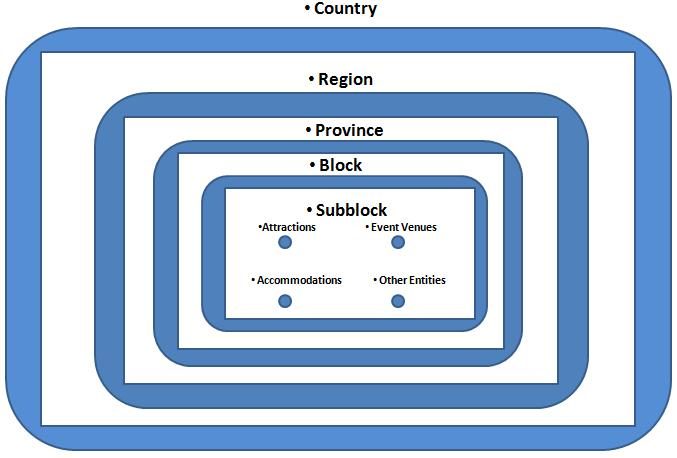
\includegraphics[width=10cm, height=7cm]{partonomy}
%\caption {Subparts of a Country}
\end{center}
\end{figure}
}


\frame{\frametitle{4.2.1.3 Excerpt from the Partonomy of Bhutan}
\begin{figure}[h] 
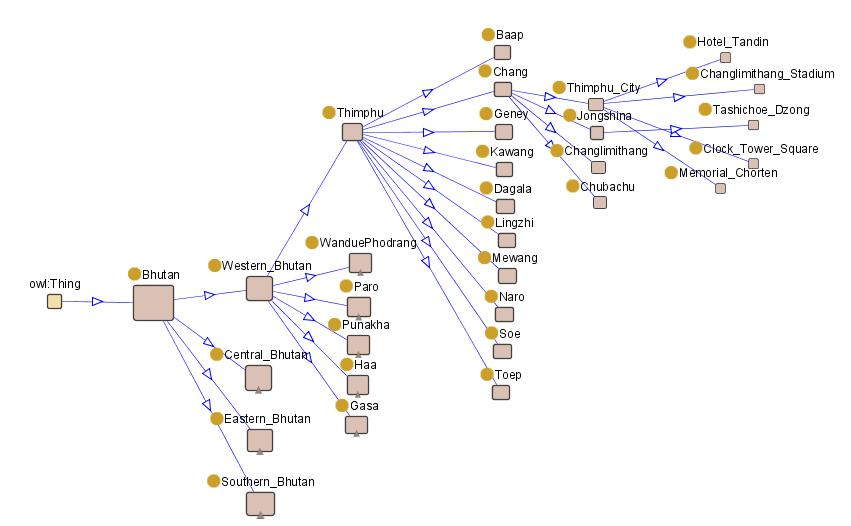
\includegraphics[width=10cm, height=7cm]{Bhutan}
\end{figure}
}

\frame{\frametitle{4.2.1.4 Partonomy KB (Ground Facts in RuleML/POSL)}
\begin{columns}[c]
\column{.565\textwidth}
 \centering
 \footnotesize
\begin{tabular}{|l|}
\hline
 \\
  \color{blue} \%siteOf(?Attraction:Attractions, ?Subblock:Subblock).\\
   siteOf(Tashichoe\_Dzong:Fortress, Jongshina:Town).\\
   siteOf(Memorial\_Chorten:Temple, Thimphu\_City:City).\\
   siteOf(Hotel\_Tandin:Hotel, Thimphu\_City:City).\\
   \\
   \\
 	\color{blue}\%partOfBlock(?Subblock:Subblock, ?Block:Block).\\
    partOfBlock(Jongshina:Town, Chang:Block).\\
    partOfBlock(Thimphu\_City:City, Chang:Block).\\
    partOfBlock(Chubachu:Town, Chang:Block).\\
    partOfBlock(Changlimithang:Town, Chang:Block).\\
    \\
    \\
  \color{blue} \%partOfProvince(?Block:Block, ?Province:Province).\\
  partOfProvince(Baap:Block, Thimphu:Province).\\
  partOfProvince(Chang:Block, Thimphu:Province).\\
 \hline
\end{tabular}
   \column{.59\textwidth}
  \centering
  \footnotesize
\begin{tabular}{|l|}
\hline
\\
  partOfProvince(Dagala:Block, Thimphu:Province).\\
  partOfProvince(Geney:Block, Thimphu:Province).\\
  partOfProvince(Kawang:Block, Thimphu:Province).\\
  partOfProvince(Lingzhi:Block, Thimphu:Province).\\
  partOfProvince(Mewang:Block, Thimphu:Province).\\
  partOfProvince(Naro:Block, Thimphu:Province).\\
  partOfProvince(Soe:Block, Thimphu:Province).\\
  partOfProvince(Toep:Block, Thimphu:Province).\\
  \\
  \\
  \color{blue} \%partOfRegion(?Province:Province, ?Region:Region).\\
   partOfRegion(Thimphu:Province, Western:Region).\\
 \\
 \\
 \color{blue} \%partOfCountry(?Region:Region, ?Country:Country).\\
  partOfCountry(Western:Region, Bhutan:Country).\\
\hline
\end{tabular}
\end{columns}
}

%%%%%%%%%%%%%%%%%%%%%%%%%%%%%%%%%%%%%%%%%%%%%%%%%%%%%%%%%%%%%%%%%%%%%%%%%%
\frame{\frametitle{4.2.1.5 Partonomy KB (Rule with Query and Result)}
\begin{figure} [tbph]
\centering
\footnotesize
\begin{tabular}{|l|}
\hline
\textbf{\color{blue}KB (Rule):}\\ 
\\
getFullAddress(?Location, [?Subblock, ?Block, ?Province, ?Region, ?Country]):-\\
\hspace{0.1in}  siteOf(?Location, ?Subblock),\\
\hspace{0.1in}    partOfBlock(?Subblock, ?Block),\\
\hspace{0.1in}   partOfProvince(?Block, ?Province),\\
\hspace{0.1in}   partOfRegion(?Province, ?Region),\\
\hspace{0.1in}    partOfCountry(?Region, ?Country).  \\
\\
\textbf{\color{blue}Sample Query:} \\ 
\\
 getFullAddress(Ta\_Dzong:National\_museum, ?Address)\\
 \\
 \textbf{\color{blue}OO jDREW TD Result:}\\
 \\
  ?Address=	[Hungrel:{\color{red}Village}, \%Subblock of type ``Village"\\
  \hspace{0.5in} Hungrel:{\color{red}Block}, \hspace{0.1in}\%Block \\
   \hspace{0.5in}Paro:Province, \\
   \hspace{0.5in}Western:Region, \\
   \hspace{0.5in}Bhutan:Country]\\
\hline
\end{tabular}
\end{figure}
}

%%%%%%%%%%%%%%%%%%%%%%%%%%%%%%%%%%%%%%%%%%%%%%%%%%%%%%%%%%%%%%%%%%%%%%%%%%
\frame{\frametitle{4.2.1.6 Search Queries and  Results}
\begin{figure} [tbph]
\centering
\footnotesize
\begin{tabular}{|l|}
\hline
 \textbf{\color{blue}Sample Queries:}\\
 \\
   1. getAttraction(?Attraction, {\color{red}Bhutan:\color{blue}Country})\\
   \\
   2. getAttraction(?Attraction, {\color{red}Western:\color{blue}Region})\\
   \\
   3. getAttraction(?Attraction, {\color{red}Bumthang:\color{blue}Province})\\
   \\
   4. getAttraction(?Attraction, {\color{red}Chhoekhor:\color{blue}Block})\\
   \\
   5. getAttraction(?Attraction, {\color{red}Chamkhar:\color{blue}Town})\\
 \\
 \\
 \textbf{\color{blue}OO jDREW TD Results for Query 5:}\\
 \\
   ?Attraction= Bumthang\_Dzong:\color{blue}Fortress\\
   ?Attraction= Zugney:\color{blue}Textiles\\
 ?Attraction=	Ugyen\_Chholing\_Museum:\color{blue}Local\_museum\\
 ?Attraction= Petseling\_Gompa:\color{blue}Temple\\
\hline
\end{tabular}
\end{figure}
}

\subsection{4.2.2 Distance Computation}
\frame{\frametitle{4.2.2 Route and Distance-time Computation}
\begin{columns}[c]
 \column{.48\textwidth}
\begin{figure}[h] 
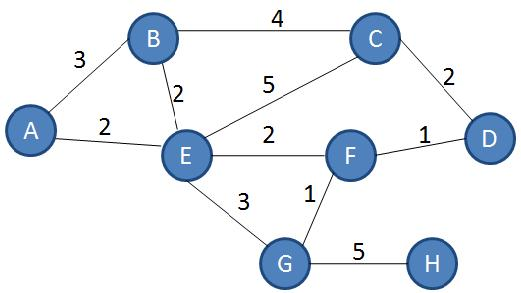
\includegraphics[width=5cm, height=4.5cm]{graph1.jpg}
\caption{A connected sample graph}
\end{figure}
\column{.64\textwidth}
\begin{figure} [tbph]
\centering
\scriptsize
\begin{table} [b]
\caption{POSL representation of the connected graph}
\begin{tabular}{|l|}
\hline                                                 
 \\
distanceTime(startPoint->A; endPoint->B; bus->3:Real).\\
distanceTime(startPoint->A; endPoint->E; bus->2:Real). \\
distanceTime(startPoint->B; endPoint->C; bus->4:Real).\\
distanceTime(startPoint->B; endPoint->E; bus->2:Real).\\
distanceTime(startPoint->E; endPoint->F; bus->2:Real). \\
distanceTime(startPoint->C; endPoint->D; bus->2:Real).\\
distanceTime(startPoint->C; endPoint->E; bus->5:Real). \\
distanceTime(startPoint->D; endPoint->F; bus->1:Real). \\	
distanceTime(startPoint->E; endPoint->G; bus->3:Real).\\
distanceTime(startPoint->F; endPoint->G; bus->1:Real). \\	
distanceTime(startPoint->G; endPoint->I; bus->5:Real). \\        
\hline
 \scriptsize {\color{blue} \textbf{KB (Rule)}}:  \\ \newline

 dTRShortest(startPoint-$>$?Province1; endPoint-$>$?Province2; \\
\hspace{0.48in}route-$>$?AllRoutes; shortestRoute-$>$?ShortestRoute):-\\
\hspace{0.1in}routeCount(startPoint-$>$?Province1; endPoint-$>$?Province2;\\
\hspace{0.5in} count-$>$?Count:Integer),\\
\hspace{0.1in}dTRList(startPoint-$>$?Province1; endPoint-$>$?Province2; \\ 
\hspace{0.37in} visited-$>$[]; currentMinRoute-$>$[R,10000:Real];\\
\hspace{0.37in} route-$>$?Routes; min-$>$?ShortestRoute; \\
\hspace{0.37in} count-$>$?Count:Integer).\\
\hline
\end{tabular}
\end {table}
\end{figure} 
\end{columns}
}

%%%%%%%%%%%%%%%%%%%%%%%%%%%%%%%%%%%%%%%%%%%%%%%%%%%%%%%%%%%%%%%%%%%%%%%%%%
\frame{\frametitle{4.2.2 Route and Distance-time Computation (Cont'd)}
\begin{figure} [tbph]
\centering
\footnotesize
\begin{tabular}{|l|}
\hline
 \textbf{\color{blue}Sample Query:}\\
    dTRShortest(startPoint-$>$A; endPoint-$>$H; \\
\hspace{0.5in}route-$>${\color{red}?AllRoutes}; \\
\hspace{0.5in}shortestRoute-$>${\color{red}?ShortestRoute})\\
 \\
 \newline
 \textbf{\color{blue}OO jDREW TD Result:}\\

  ?AllRoutes= [[[A, E, G, H], 10.0:Real], \\ \newline 
   \hspace{0.54in}   [[A, B, E, G, H], 13.0:Real], \\  \newline
    \hspace{0.54in}  [[A, E, F, G, H], 10.0 : Real], \\ \newline 
   \hspace{0.54in} [[A, B, C, E, G, H], 20.0 : Real],\\  \newline 
		\hspace{0.54in} [[A, B, E, F, G, H], 13.0 : Real], \\ \newline 
		\hspace{0.54in} [[A, B, C, D, F, G, H], 16.0 : Real],\\ \newline 
		\hspace{0.54in} [[A, B, C, E, F, G, H], 20.0 : Real], \\ \newline 
		\hspace{0.54in} [[A, E, C, D, F, G, H], 16.0 : Real], \\ \newline 
		\hspace{0.54in} [[A, B, C, D, F, E, G, H], 20.0 : Real],\\ \newline 
		\hspace{0.54in}  [[A, B, E, C, D, F, G, H], 19.0 : Real], \\ \newline 
		\hspace{0.54in} [[A, E, B, C, D, F, G, H], 17.0 : Real]]\\ 
	?ShortestRoute=  [[A, E, G, H], 10.0 : Real]\\ 							 
   \hline
\end{tabular}
\end{figure}
}
%%%%%%%%%%%%%%%%%%%%%%%%%%%%%%%%%%%%%%%%%%
\subsection{4.3.1 Rule System for eTourPlan Attraction-only Travel Planner}
\frame{\frametitle{4.3.1 Rule System for eTourPlan Attraction-only Planning}
\begin{columns}[c]
 \column{.595\textwidth}
\hspace{0.1cm}{\textbf{\color{blue} The planner performs the following steps}}:
 \vspace{0.1in}
 \pause
\begin{enumerate}
\item From the user-specified starting point, an attraction is selected and chains to the next
      related attraction.
 \vspace{0.2in}   
 \pause  
\item Compute and validate route and travel-time constrained
      by global constants:
\vspace{0.1in}
{\footnotesize \hspace{0.04in} -maxActivitySightSeeingHoursInADay(12:Real)}\\
{\footnotesize \hspace{0.04in} -maxHoursAtAnAttractionSite(4:Real)}\\

\vspace{0.2in}
\pause
\item On successful validation of distance and remaining time, 
      add detailed information of the selected attraction to the
      travel plan.\\
\end{enumerate}
\column{.72\textwidth}
\begin{figure}
%\raggedright
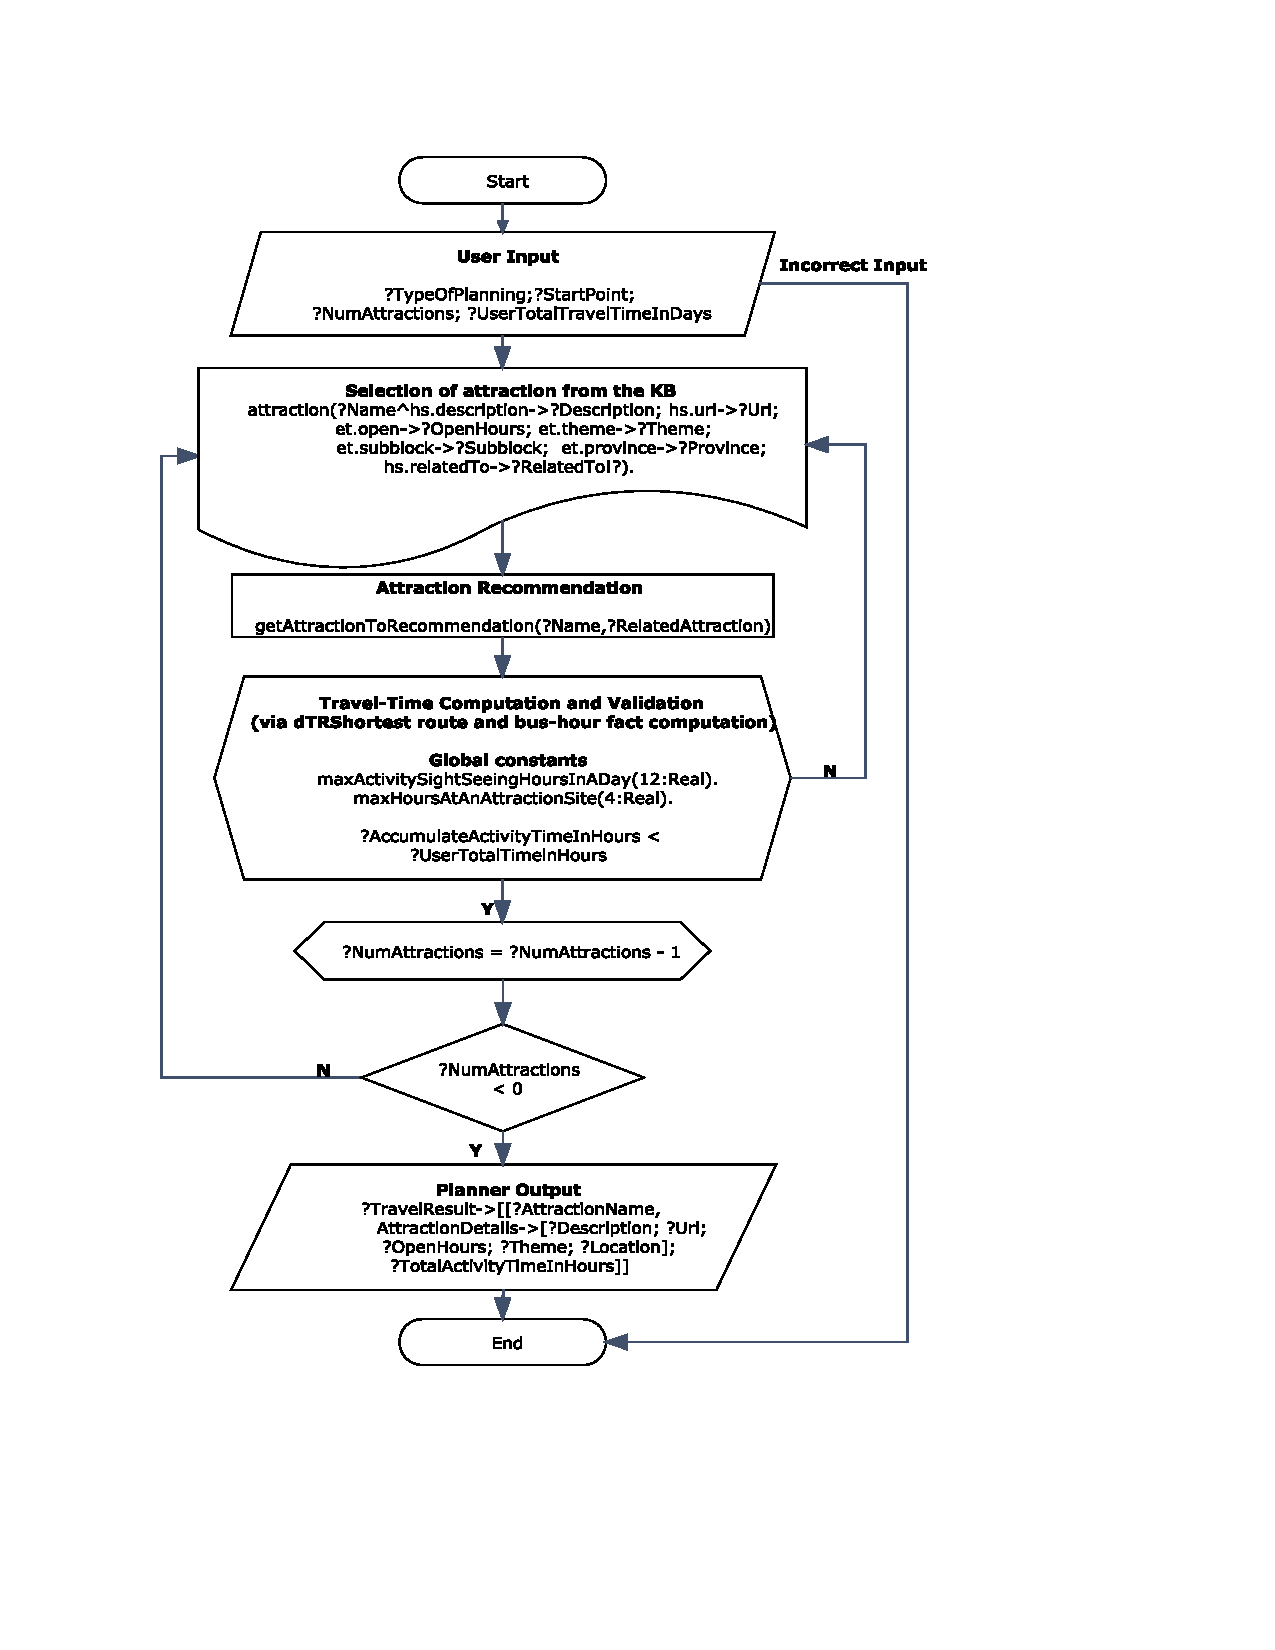
\includegraphics[width=5cm, height=7cm]{eTourPlanA.pdf}
\end{figure}
\end{columns}
}

%%%%%%%%%%%%%%%%%%%%%%%%%%%%%%%%%%%%%%%%%%%%%%%%%%%%%%%%%%%%%%%%%
\subsection{4.3.2 Rule System for eTourPlan Travel Planner}
\frame{\frametitle{4.3.2 Rule System for eTourPlan Event-centric Planning}
\begin{columns}[c]
\column{.55\textwidth}
\hspace{0.08cm}{\color{blue}The planner performs the following steps}:
 \vspace{0.2in}
\footnotesize
\begin{enumerate}
\pause
\item Events are selected by validating the event dates \\
      against the user's travel dates, minimum break,\\
      and maximum break.
 \vspace{0.2in} 
\pause    
\item Compute and validate route and bus hours constrained
      by maximum break. 
\pause
\vspace{0.2in}
\item On successful validation of distance
and remaining time, add detailed information
of the selected event to the travel plan.
\vspace{0.2in}
\pause     
\item Recommend attractions located in the subblock of the
      selected event. 
\pause      
\vspace{0.2in}     
\item Provide on-route attraction recommendation
if the user selects the option (constrained by the
global constant ``maxTimeGapBetweenEvents").    
\end{enumerate}
 \column{.75\textwidth}
\begin{figure}
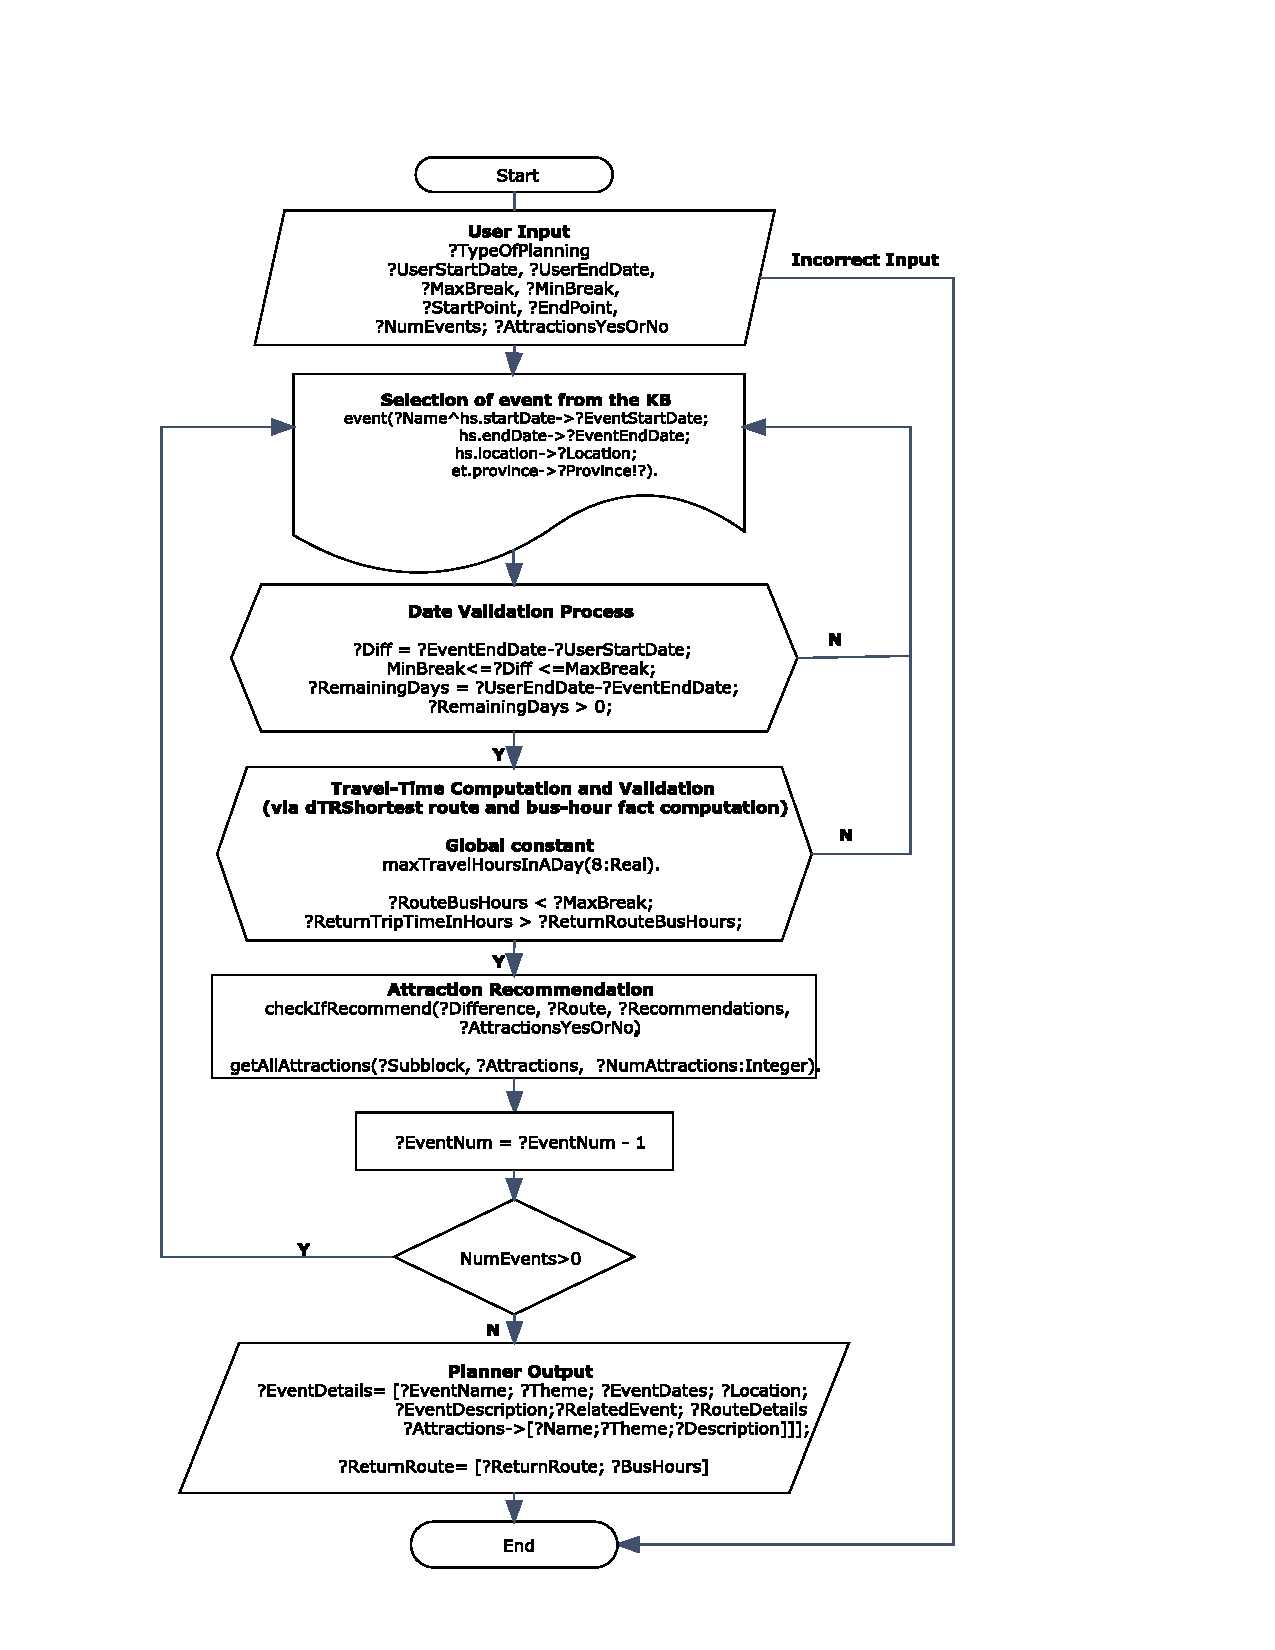
\includegraphics[width=5.3cm, height=7.5cm]{eTourPlanE.pdf}
\end{figure}
\end{columns}
}

\section{5. Experimental Results}
\subsection{5.1 Parametric Search Operations}
\frame{\frametitle{5.1.1 Parametric Search Operations}
%\textbf{\color{blue}5.1. Search Operations:}\vspace{0.2cm}
\pause
\begin{enumerate}
\item Search for Provincial Information
 \begin{itemize}
\item {\color{blue}name
\item region
}
\end{itemize}
\vspace{0.1cm}
\pause
\item Search for Route Information 
 \begin{itemize}
\item {\color{blue}startPoint, endPoint
\item list of user-specified provinces}
\end{itemize}
\vspace{0.1cm}
\pause
\item Search for Activities (Events and Attractions)
 \begin{itemize}
\item {\color{blue}name:type
\item \_:type {\scriptsize {\color{black}(refers to the classification of activity)}}
\item theme
}
\end{itemize}
at {\color{red} {\footnotesize(Subblock, Block, Province, Region, Country)}} of Partonomy
\vspace{0.2cm}
\pause
\item Search for Accommodations\vspace{0.1cm}
 \begin{itemize}
\item {\color{blue}name:type {\scriptsize {\color{black}(refers to the type of accommodation)}}
\item \_:type
\item price
}
\end{itemize}
at {\color{red} {\footnotesize(Subblock, Block, Province, Region, Country)}} of Partonomy
\end{enumerate}
}

\frame{\frametitle{5.1.2 Sample Activity Search Query and Result}
\begin{table} [tbph]
%\caption{Query mode (input/output) for Route search}
\centering
\footnotesize
\begin{tabular}{|l|}
\hline
$~~~~~~~~~~~~~~~~~~~~~~~~~~~~~~$Query\\
\hline
getActivityDetails(actName-$>?$Name:\textbf{{\color{blue}Events}};\\
$~~~~~~~~~~~~~~~~~~~~~~~~~~~~~~$theme-$>$\textbf{{\color{blue}Recreation}}; \\        $~~~~~~~~~~~~~~~~~~~~~~~~~~~~~~$address-$>$[?Subblock, \\
$~~~~~~~~~~~~~~~~~~~~~~~~~~~~~~~~~~~~~~~~~~~~~~~?$Block, \\
$~~~~~~~~~~~~~~~~~~~~~~~~~~~~~~~~~~~~~~~~~~~~~~~?$Province,\\
$~~~~~~~~~~~~~~~~~~~~~~~~~~~~~~~~~~~~~~~~~~~~~~$\textbf{{\color{blue}Southern:Region}}, \\
$~~~~~~~~~~~~~~~~~~~~~~~~~~~~~~~~~~~~~~~~~~~~~~~?$Country]; \\
$~~~~~~~~~~~~~~~~~~~~~~~~~~~~~${\color{red}$?$ActivityDetails})\\ 
\hline
\end{tabular} 
\end{table}

\pause \begin{table} [tbph]
%\caption{Route search result for Query 1}
\centering
\footnotesize
\begin{tabular}{|l|l|}
\hline
 \textbf{Output} &$~~~~~~~~~~~~~~~~~~~~~~~~~~$\textbf{Variable Bindings} \\
 \textbf{Variables}& $~~~~~~~~~~~~~~~~~~~~~~~~~~~~~~$\\
\hline
 {\color{red}$?$ActivityDetails}&[ActName-$>$Yangphel\_Archery\_Tournament:Sport\_archery;\\
           &$~$WebLink-$>$``{\color{red}http://www.bhutanarchery.com/default.asp}"; \\
		   &$~$EventDates-$>$[StartDate-$>$date[2008:Real, 08:Real, 23:Real];\\
           &$~~~~~~~~~~~~~~~~~~~~~~~~$EndDate-$>$date[2008:Real, 10:Real, 02:Real]];\\	   
          &$~$Description-$>$``11TH Yangphel open archery tournament";\\
          &$~$Address-$>$[Phuentsholing\_Upper\_Town:Town, \\
		&$~~~~~~~~~~~~~~~~~~~$Phuentsholing:Block, \\
		&$~~~~~~~~~~~~~~~~~~~$Chukha:Province, \\
		&$~~~~~~~~~~~~~~~~~~~$Southern:Region,\\
        &$~~~~~~~~~~~~~~~~~~~$Bhutan:Country];\\
		&$~$Theme-$>$Recreation;\\
        &$~$RelatedTo-$>$``Thimphu\_Drupchen:Annual\_festival"] \\
\hline
\end{tabular} 
\end{table}
}


\subsection{5.2. Location-centric Recommender}
\frame{\frametitle{5.2.1 Location-centric Recommender}
\begin{itemize}
\item Provides route and tourism information for 
\begin{enumerate}
\item {\color{blue} SystemRecommendation}: Number of `N' ``relatedTo" provinces
\item {\color{blue} UserPrefBased}: User-specified list of provinces
\end{enumerate}
\end{itemize}
\vspace{0.1in}
\begin{table} [tbph]
\centering
\footnotesize
\centering
\begin{tabular}{|l|l|l|}
\hline
 &\textbf{User Input} &$~~~~~~~~~~~~~~~~~~~~$ \textbf{Query Formats} \\
 &$~~$\textbf{Values}   &$~~~~~~~~~~~~$(Input values are blue bold-faced)          \\
\hline
  1&typeOfRecommend & locCentricRecommend(typeOfRecommend-$>$\\
     &numProvinces        &$~~~~~~~~~~~~~~~~~~~~~~~~~~~~~~~~~~~~~$\textbf{{\color{blue}SystemRecommendation}};\\
     & &$~~~~~~$userInputs-$>$[startPoint-$>$\textbf{{\color{blue}Paro:Province}}; \\
     & &$~~~~~~~~~~~~~~~~~~~~~~~~~~~$numProvinces-$>$\textbf{{\color{blue}3:Integer}}]; \\
         &                       &$~~~~~~${\color{red}[$?$Routes, $?$Recommendations, $?$TotalBusHours]}) \\          
\hline
 2&typeOfRecommend & locCentricRecommend(typeOfRecommend-$>$\textbf{{\color{blue}UserPrefBased}};\\
  &startPoint       &$~~~~~~$userInputs-$>$[startPoint-$>$\textbf{{\color{blue}Paro:Province}}; \\
  &userPrefList     &$~~~~~~~~~~~~~~~~~~~~~~~~~~~~$userPrefList-$>$\textbf{{\color{blue}[Chukha:Province]}};\\
  &endPoint         &$~~~~~~~~~~~~~~~~~~~~~~~~~~~~$endPoint-$>$\textbf{{\color{blue}Thimphu:Province}}]; \\
  &                       &$~~~~~~${\color{red}[$?$Routes, $?$Recommendations, $?$TotalBusHours]})\\  
\hline      
\end{tabular} 
\caption{Queries of different input/output modes for location-centric Recommendation}
\end{table}
}


\frame{\frametitle{5.2.2 Recommendation Results for Query 2}
\begin{table} [tbph]
\caption{Location-centric recommendation for user-preferred Provinces}
\centering
\scriptsize
\begin{tabular}{|l|l|}
\hline
 \textbf{Output} &$~~~~~~~~~~~~~~~~~~~~~~~~~~$\textbf{Variable Bindings} \\
 \textbf{Variables}&  $~~~~~~~~~~~~~~~~~~~~~~~~~~~~~~$(For Query 2)              \\
 \hline
{\color{red} $?$Routes } &[[Paro, Chuzom, Chukha], 6.5 :Real,\\
           &$~$[Chukha, Chuzom, Thimphu], 7.0 :Real]\\
 {\color{red}$?$Recommendations}&[Chukha; \\
                   &\cellcolor{yellow}EventList-$>$\\
  				   &$~~~~$[[EventName-$>$Chukha\_Tshechu:Annual\_festival;\\
				   &$~~~~~~$Description-$>$``One of the most amazing festivals in Chukha";\\
				   &$~~~~~~$Address-$>$[Chukha\_Town:Town, \\
		           &$~~~~~~~~~~~~~~~~~~~~~~~~~$Gelling:Block, \\
		           &$~~~~~~~~~~~~~~~~~~~~~~~~~$Southern:Region, \\
		           &$~~~~~~~~~~~~~~~~~~~~~~~~~$Bhutan:Country,\\
                 &$~~~~~~$EventDates-$>$[StartDate-$>$date[2008:Real, 03:Real, 19:Real];\\
                &$~~~~~~~~~~~~~~~~~~~~~~~~~~~~~~$EndDate-$>$date[2008:Real, 03:Real, 21:Real]]],\\	   
                  &$~~~~~$[EventName-$>$Yangphel\_Archery\_Tournament:Sport\_archery;\\
				   &$~~~~~~$Description-$>$``11TH Yangphel open archery tournament";\\
				   &$~~~~~~$Address-$>$[Phuentsholing\_Upper\_Town:Town, \\
		         &$~~~~~~~~~~~~~~~~~~~~~~~~~$Phuentsholing:Block,, \\
		          &$~~~~~~~~~~~~~~~~~~~~~~~~~$Southern:Region, \\
		           &$~~~~~~~~~~~~~~~~~~~~~~~~~$Bhutan :Country,\\
                 &$~~~~~~$EventDates-$>$[StartDate-$>$date[2008:Real, 08:Real, 23:Real];\\
             &$~~~~~~~~~~~~~~~~~~~~~~~~~~~~~~$EndDate-$>$date[2008:Real, 10:Real, 02 :Real]]]]; \\	   
\end{tabular} 
\end{table}
}

\frame{\frametitle{5.2.2 Recommendation Results (Cont'd)}
\begin{table} [tbph]
\footnotesize
%\caption{Location-centric recommendation for user-preferred Provinces}
\centering
%\footnotesize
\scriptsize
\begin{tabular}{|l|l|}
%\hline 
% \textbf{Output} &$~~~~~~~~~~~~~~~~~~~~~~~~~~$\textbf{Variable Bindings} \\
% \textbf{Values}& \\
% \hline 
 {\color{red}$?$Recommendations} &\cellcolor{yellow}AttractionList-$>$ \\
  				   &$~~~~$[[AttractionName-$>$Chukha\_Dzong:Fortress;\\
				   &$~~~~~~$WebLink-$>$`` "; \\
				   &$~~~~~~$Description-$>$``It is one of the most beautiful attractions.";\\      
		       &\cellcolor{yellow}AccommodationList-$>$\\
  				   &$~~~~$[[Hotel\_Druk\_Phuentsholing:Hotel; \\
			       &$~~~~~~$WebLink-$>$``www.drukhotels.com/"; \\
                   &$~~~~~~$MinPrice-$>$"2700:Real";\\
				   &$~~~~~~$Rating-$>$4:Real], \\
		           &$~~~~$[Hotel\_Namgay:Hotel;  \\
			       &$~~~~~~$WebLink-$>$``www.hotelNamgay.bt/"; \\
                   &$~~~~~~$MinPrice-$>$"1800:Real";\\
				   &$~~~~~~$Rating-$>$3:Real]]]] \\	
 \hline
		  {\color{red}$?$TotalBusHours}  &13.5:Real\\	
\hline   
\end{tabular} 
\end{table}
}

\subsection{5.3. eTourPlan Travel Planner}
\frame{\frametitle{5.3.1 eTourPlan Travel Planner}
\vspace{0.05in}
\begin{itemize}
\item {\color{blue}Two modes of Travel Planning}:
\begin{enumerate}
\item {\color{blue}AttractionOnly}: Based on ``relatedTo" attractions
\item {\color{blue}EventCentric}: Based on temporal-geographic search criteria
\end{enumerate}
\end{itemize}
\vspace{0.05in}

\begin{table} [tbph]
\centering
\scriptsize
\begin{tabular}{|l|l|l|}
\hline
 &\textbf{User Input} &$~~~~~~~~~~~~~~~~~~~~$ \textbf{Query Formats} \\
 &$~~$\textbf{Values}   & $~~~~~~~~~~~~$(Input values are bold-faced)   \\
\hline
 1&typeOfPlanning &eTourPlan(typeOfPlanning-$>${\color{blue}\textbf{AttractionOnly}};\\
  &startPoint     &$~~~$userInputs-$>$[startPoint-$>${\color{blue}\textbf{Paro:Province}}; \\
  &endPoint         &$~~~~~~~~~~~~~~~~~~~~$endPoint-$>${\color{blue}\textbf{Thimphu:Province}}; \\
  &numAttractions   &$~~~~~~~~~~~~~~~~~~~~$numAttractions-$>${\color{blue}\textbf{4}:Integer};\\ &userTotalTravelTimeInDays&$~~~~~~~~~~~~~~~~~~~$userTotalTravelTimeInDays-$>${\color{blue}\textbf{4}:Integer}];\\
  &                       &$~~~${\color{red}$?$TravelResult}) \\        
\hline
2&typeOfPlanning & eTourPlan(typeOfPlanning-$>${\color{blue}\textbf{EventCentric}};\\
   &                        &$~$userInputs-$>$[\\
   &startPoint          &$~~~$startPoint-$>${\color{blue}\textbf{Paro:Province}}; \\
  &endPoint       &$~~~$endPoint-$>${\color{blue}\textbf{Thimphu:Province}}; \\
  &userStartDate  &$~~~$userStartDate-$>${\color{blue}\textbf{date[2008:Real,10:Real,01:Real]}}; \\
  &userEndDate    &$~~~$userEndDate-$>${\color{blue}\textbf{date[2008:Real,11:Real,10:Real]}}; \\
  &maxBreak       &$~~~$maxBreak-$>${\color{blue}\textbf{10:Real}}; \\
  &minBreak       &$~~~$minBreak-$>${\color{blue}\textbf{0:Real}}; \\
  &attractionRecommendation&$~~~$attractionRecommendation-$>${\color{blue}\textbf{No}}; \\
  &eventNum      &$~~~$eventNum-$>${\color{blue}\textbf{3:Integer}}]; \\
  &                      &$~${\color{red}$?$TravelResult})\\         
\hline
\end{tabular} 
\caption{Queries of different input/output modes for Travel Planning}
\end{table}
}

\frame{\frametitle{5.3.2 Travel Planning Scenario}

{\large \emph{{\color{blue}User queries for an event-centric plan of {\color{red}3 events} between the {\color{red}1st of October and the 10th of November} and specifies a {\color{red}``maxBreak"} of {\color{red}10 days} and {\color{red}``minBreak"} of {\color{red}0 days} between main events. User also specifies the starting province,`` {\color{red}Paro:Province}", and the final destination province, as ``{\color{red}Thimphu:Province}". User checks {\color{red}``No"} for on-route attraction recommendation, knowing that the planner provides recommendation of attractions at the subblock of event location.}}}}

\frame{\frametitle{5.3.3 Event Schedules}
\begin{table} [tbph]
\footnotesize
\caption{Evaluation of event-centric travel results}
\centering
\begin{tabular}{|l|l|l|}
\hline
Event &Event Schedules &Event Sequences\\
 & & $~~~~~$of length\\
 & &$~$ ?EventNum= 3\\
\hline
{\textbf{\color{blue}  1}}  &Tamshingphala\_Choepa:Traditional\_festival&\textbf{{\color{blue} 1},{\color{blue} 2},{\color{blue} 5}}\\
     &startDate-$>$date[2008:Real,10:Real,08:Real]&\\
   &endDate-$>$date[2008:Real,10:Real,10:Real]&\\
   &province-$>$Bumthang&\\
\hline
{\textbf{\color{blue} 2}}  &Tangbi\_Mani:Traditional\_festival&\\
     &startDate-$>$date[2008:Real,10:Real,13:Real]&\\
   &endDate-$>$date[2008:Real,10:Real,15:Real]&\\
   &province-$>$Bumthang&\\
\hline
{\textbf{\color{blue} 3}}  &Thimphu\_Drupchen:Annual\_festival&\textbf{{\color{blue} 3},{\color{blue} 2},{\color{blue} 5}}\\
     &startDate-$>$date[2008:Real,10:Real,04:Real]&\textbf{{\color{blue} 3},{\color{blue} 4},{\color{blue} 2}}\\
   &endDate-$>$date[2008:Real,10:Real,08:Real]&\textbf{{\color{blue} 3},{\color{blue} 4},{\color{blue} 5}}\\
   &province-$>$Thimphu&\\
\hline
{\textbf{\color{blue} 4}}  &Thimphu\_Tshechu:Annual\_festival&\textbf{{\color{blue} 4},{\color{blue} 2},{\color{blue} 5}}\\
     &startDate-$>$date[2008:Real,10:Real,09:Real]&\\
   &endDate-$>$date[2008:Real,10:Real,11:Real]&\\
   &province-$>$Thimphu&\\
\hline
{\textbf{\color{blue} 5}}  &Wangdue\_Tshechu:Annual\_festival&\\
     &startDate-$>$date[2008:Real,10:Real,20:Real]&\\
   &endDate-$>$date[2008:Real, 10:Real, 29:Real]&\\
   &province-$>$WangduePhodrang&\\
\hline
\end{tabular} 
\end{table} 
}

\frame{\frametitle{5.3.4 Multiple Travel Plans}
\begin{table} [tbph]
\footnotesize
\caption{Options for event-centric travel plans}
\centering
\begin{tabular}{|l|l|l|}
\hline
\textbf{\color{blue} Option} &\textbf{\color{blue}Event Sequences of length ``3"}&\textbf{\color{blue}Province}\\
                
\hline
\rowcolor{yellow}
 1&Tamshingphala\_Choepa:Traditional\_festival& Bumthang\\
 \rowcolor{yellow}
  &Tangbi\_Mani:Traditional\_festival&Bumthang\\
 \rowcolor{yellow}
  &Wangdue\_Tshechu:Annual\_festival&WangduePhodrang\\
  \rowcolor{yellow}
  &                                 &   \\
\hline
 2&Thimphu\_Drupchen:Annual\_festival&Thimphu\\
  &Tangbi\_Mani:Traditional\_festival&Bumthang\\
  &Wangdue\_Tshechu:Annual\_festival&WangduePhodrang\\
  &                                 &   \\
\hline
 3&Thimphu\_Drupchen:Annual\_festival&Thimphu\\
  &Thimphu\_Tshechu:Annual\_festival &Thimphu\\
  &Tangbi\_Mani:Traditional\_festival&Bumthang\\
  &                                 &   \\
\hline
\rowcolor{yellow}
 4&Thimphu\_Drupchen:Annual\_festival&Thimphu\\
\rowcolor{yellow} 
  &Thimphu\_Tshechu:Annual\_festival&Thimphu\\
\rowcolor{yellow}
  &Wangdue\_Tshechu:Annual\_festival&WangduePhodrang\\
\rowcolor{yellow}
  &                                 &   \\
\hline
 5&Thimphu\_Tshechu:Annual\_festival&Thimphu\\
  &Tangbi\_Mani:Traditional\_festival&Bumthang\\
  &Wangdue\_Tshechu:Annual\_festival&WangduePhodrang\\
  &                                 &   \\
\hline
\end{tabular} 
\end{table} 
}


\frame{\frametitle{5.3.5 Complete Result of the First Travel Plan Option (Events 1, 2 and 5)}
\begin{table} [tbph]
\caption{Event-centric travel results}
\centering
\scriptsize
\begin{tabular}{|l|l|}
\hline
 \textbf{Output} &$~~~~~~~~~~~~~~~~~~~~~~~~~~$\textbf{Variable Bindings} \\
 \textbf{Variables}&                \\
\hline
 {\color{red}$?$TravelResult}&\cellcolor{yellow}[[[EventName-$>$Tamshingphala\_Choepa:Traditional\_festival;\\
  		 &$~~~$EventDates-$>$[Startdate-$>$date[2008:Real, 10:Real, 08:Real];\\
		    &$~~~~~~~~~~~~~~~~~~~~~~~~~~$Enddate-$>$date[2008:Real, 10:Real, 10:Real]];\\
			  &$~~~$Theme-$>$Cultural\_Religious\_Heritage;\\
			  &$~~~$EventDescription-$>$``One of the most amazing festivals in Bumthang"\\
		  	  &$~~~$Location-$>$[Tamshing\_Lhakhang:Temple, \\
		  	  &$~~~~~~~~~~~~~~~~~~~~~$Tamshing\_Village:Village,\\ 
		  	  &$~~~~~~~~~~~~~~~~~~~~~$Bumthang:Province];\\
			  &$~~~$RelatedEvent-$>$Tangbi\_Mani:Traditional\_festival;\\
			&$~~~${\color{blue}RouteDetails}-$>$[[Paro:Province, Chuzom:Province, Thimphu:Province,\\
      &$~~~~~~~~~~~~~~~~~~~~~~~~~~~~~$Lobesa:Province, WangduePhodrang:Province, \\ 
			&$~~~~~~~~~~~~~~~~~~~~~~~~~~~~~$Trongsa:Province, Bumthang:Province], \\
			&$~~~~~~~~~~~~~~~~~~~~~~~~~~~~~$[]; RouteBusHours-$>$16.7:Real];\\
			 &$~~~${\color{blue}RecommendedAttractions}-$>$[Tamshing\_Lhakhang:Temple, \\
		   &$~~~~~~~~~~~~~~~~~~~~~~~~~~~~~~~~~~~~$``It was built by Pema Lingpa,the Treasure Revealer in 1505."]],\\
		   &$~~~$\cellcolor{yellow}[EventName-$>$Tangbi\_Mani:Traditional\_festival;\\
  		 &$~~~$EventDates-$>$[Startdate-$>$date[2008:Real, 10:Real, 13:Real;\\
		    &$~~~~~~~~~~~~~~~~~~~~~~~~~~$Enddate-$>$date[2008:Real, 10:Real, 15:Real]];\\
			  &$~~~$Theme-$>$Cultural\_Religious\_Heritage;\\
			  &$~~~$EventDescription-$>$``A prestigious annual festival in Bumthang"\\
		  	  &$~~~$Location-$>$[Tangbi\_Monastery:Monastery, \\
		  	  &$~~~~~~~~~~~~~~~~~~~~~~$Tangbi:Village,\\ 
		  	  &$~~~~~~~~~~~~~~~~~~~~~~$Bumthang:Province];\\
			  &$~~~$RelatedEvent-$>$Wangdue\_Tshechu:Annual\_festival; \\
\end{tabular} 
\end{table}						
}


\frame{\frametitle{5.3.5 Detailed Result of a Travel Plan (Cont'd)}
\begin{table} [tbph]
\footnotesize
%\caption{Event-centric travel result}
\centering
\scriptsize
\begin{tabular}{|l|l|}
%\hline 
% \textbf{Output} &$~~~~~~~~~~~~~~~~~~~~~~~~~~$\textbf{Variable Bindings} \\
% \textbf{Values}& \\
 %\hline            
 		{\color{red}$?$TravelResult}
 			&$~~~${\color{blue}RouteDetails}-$>$[[Bumthang:Province],  \\
      &$~~~~~~~~~~~~~~~~~~~~~~~~~~~~$[]; RouteBusHours-$>$0:Real]]; \\ 
									
		   &$~~~${\color{blue}RecommendedAttractions}-$>$[Tangbi\_Monastery:Monastery \\
		   &$~~~~~~~~~~~~~~~~~~~~~~~~~~~~~~~~~~~~$``Located in upper Tang valley."]],\\	   
 		   &$~~~$\cellcolor{yellow}[EventName-$>$Wangdue\_Tshechu:Annual\_festival;\\
  		 &$~~~$EventDates-$>$[Startdate-$>$date[2008:Real, 10:Real, 20:Real];\\
		    &$~~~~~~~~~~~~~~~~~~~~~~~~~~$Enddate-$>$date[2008:Real, 10:Real, 29:Real]];\\
			  &$~~~$Theme-$>$Cultural\_Religious\_Heritage;\\
			  &$~~~$EventDescription-$>$``A very popular festival in western Bhutan"\\
		  	  &$~~~$Location-$>$[Wangdue\_Dzong:Fortress, \\
		  	  &$~~~~~~~~~~~~~~~~~~~~~~$Wangdue\_Town:Town,\\ 
		  	  &$~~~~~~~~~~~~~~~~~~~~~~$WangduePhodrang:Province];\\
		  	  &$~~~${\color{blue}RouteDetails}-$>$[[Bumthang:Province, Trongsa:Province,  \\   
	       &$~~~~~~~~~~~~~~~~~~~~~~~~~~~~$WangduePhodrang:Province], [];  \\
         &$~~~~~~~~~~~~~~~~~~~~~~~~~~~~$[]; RouteBusHours-$>$0:Real]; \\ 			
		   &$~~~${\color{blue}RecommendedAttractions}-$>$[Wangdue\_Dzong:Fortress \\
		   &$~~~~~~~~~~~~~~~~~~~~~~~~~~~~~~~~~~~~$``It is one of the most beautiful attractions."]],\\	   
     &$~~${\color{blue}ReturnRoute}-$>$[[WangduePhodrang:Province, Lobesa:Province, \\
	   &$~~~~~~~~~~~~~~~~~~~~~~~~~~~~$Thimphu:Province]; Returntime-$>$12.2:Real]]\\
\hline	
\end{tabular} 
\end{table}
} 


\frame{\frametitle{5.3.6 Travel Plan (Option 4) -At the starting point}
\begin{figure}
\centering
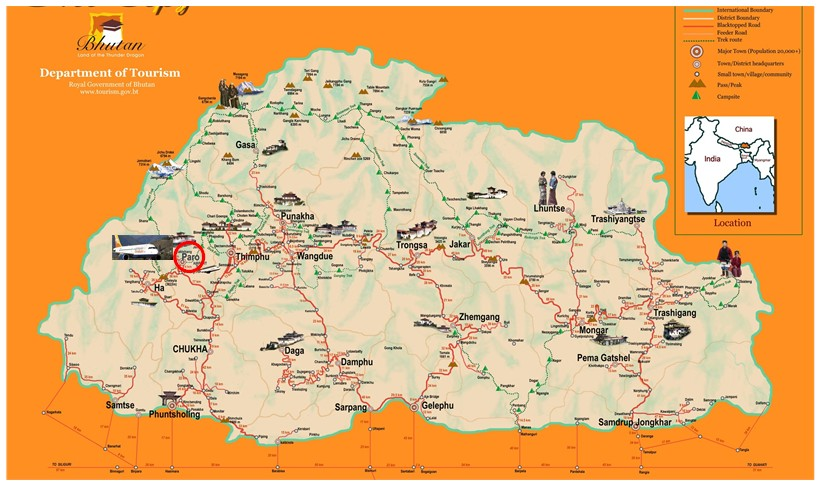
\includegraphics[width=11.5cm, height=7cm]{E1}
\caption{Travel Planning Scenario}
\end{figure}}

\frame{\frametitle{5.3.6 Travel Plan -Event 1 found}
\begin{figure}
\centering
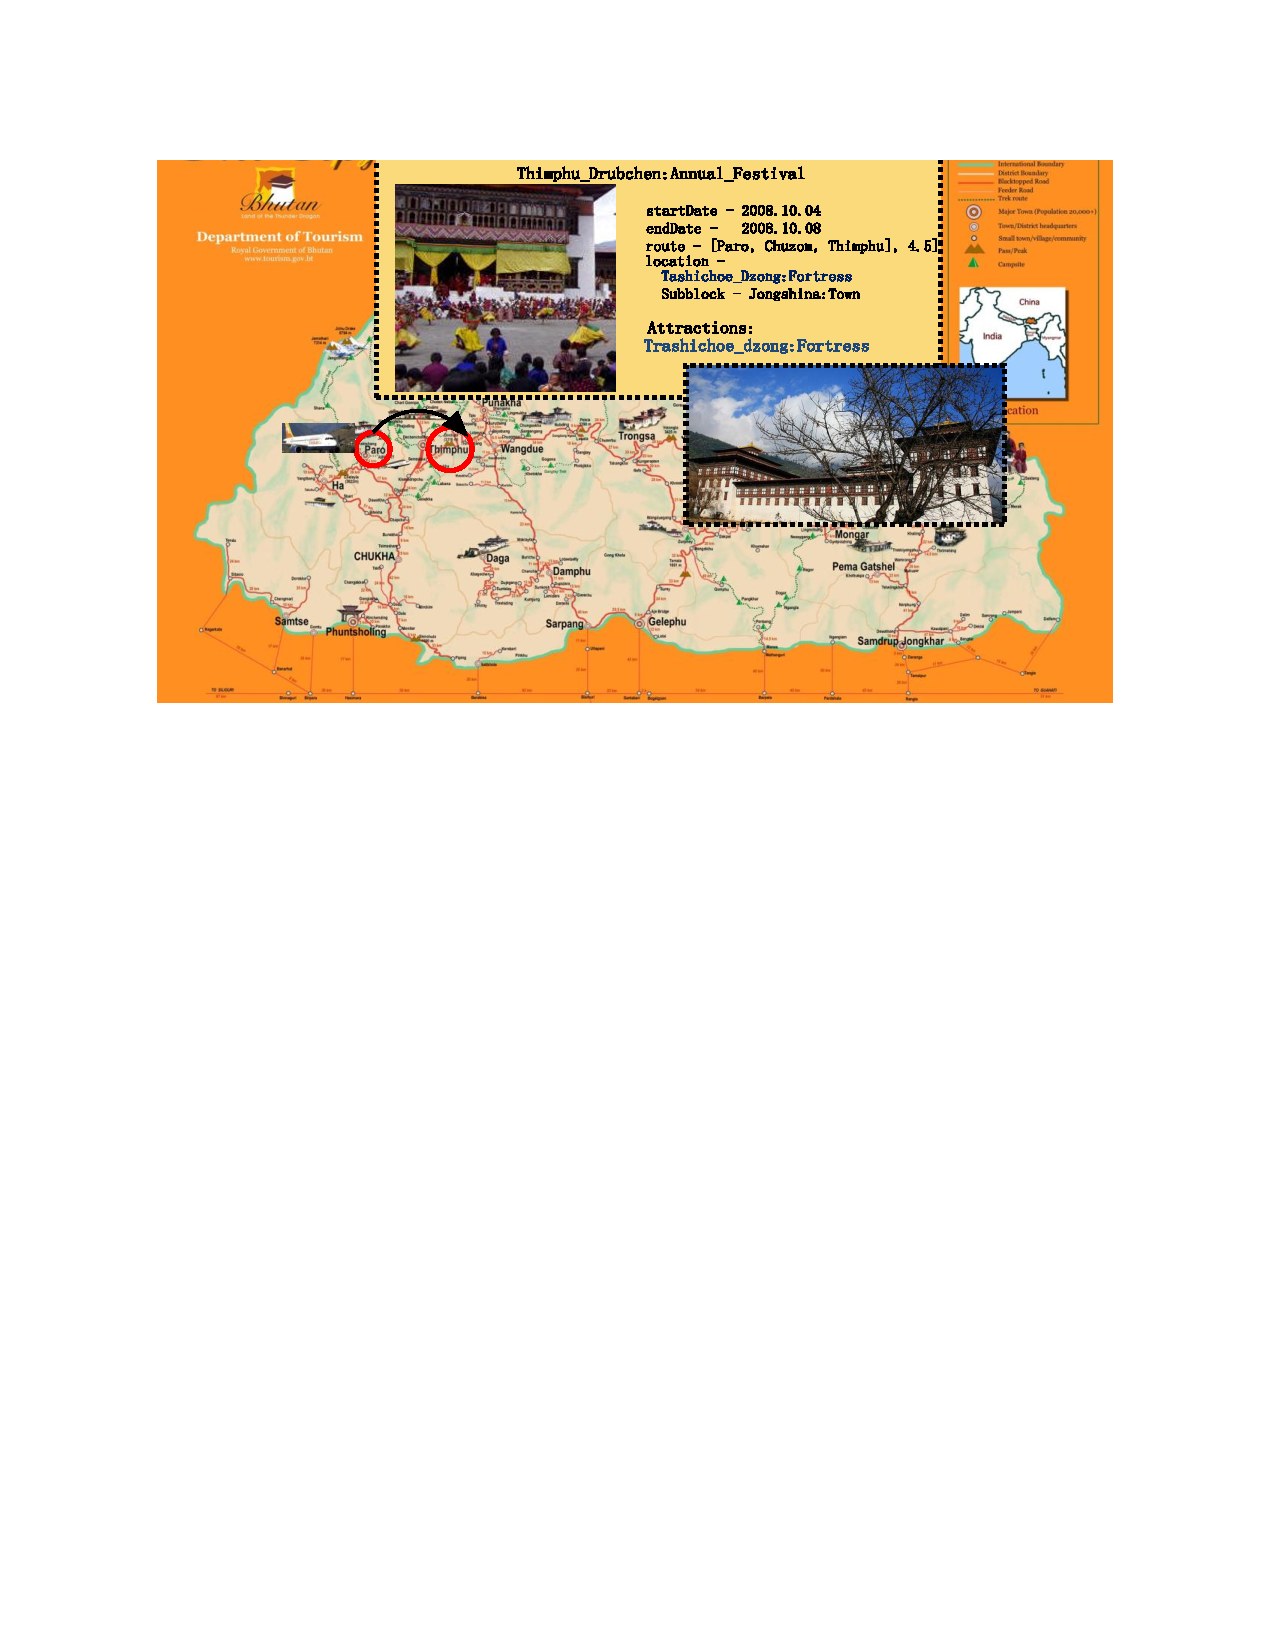
\includegraphics[width=11.5cm, height=7cm]{E2}
\caption{Travel Planning Scenario}
\end{figure}}
\frame{\frametitle{5.3.6 Travel Plan -Event 2 found}
\begin{figure}
\centering
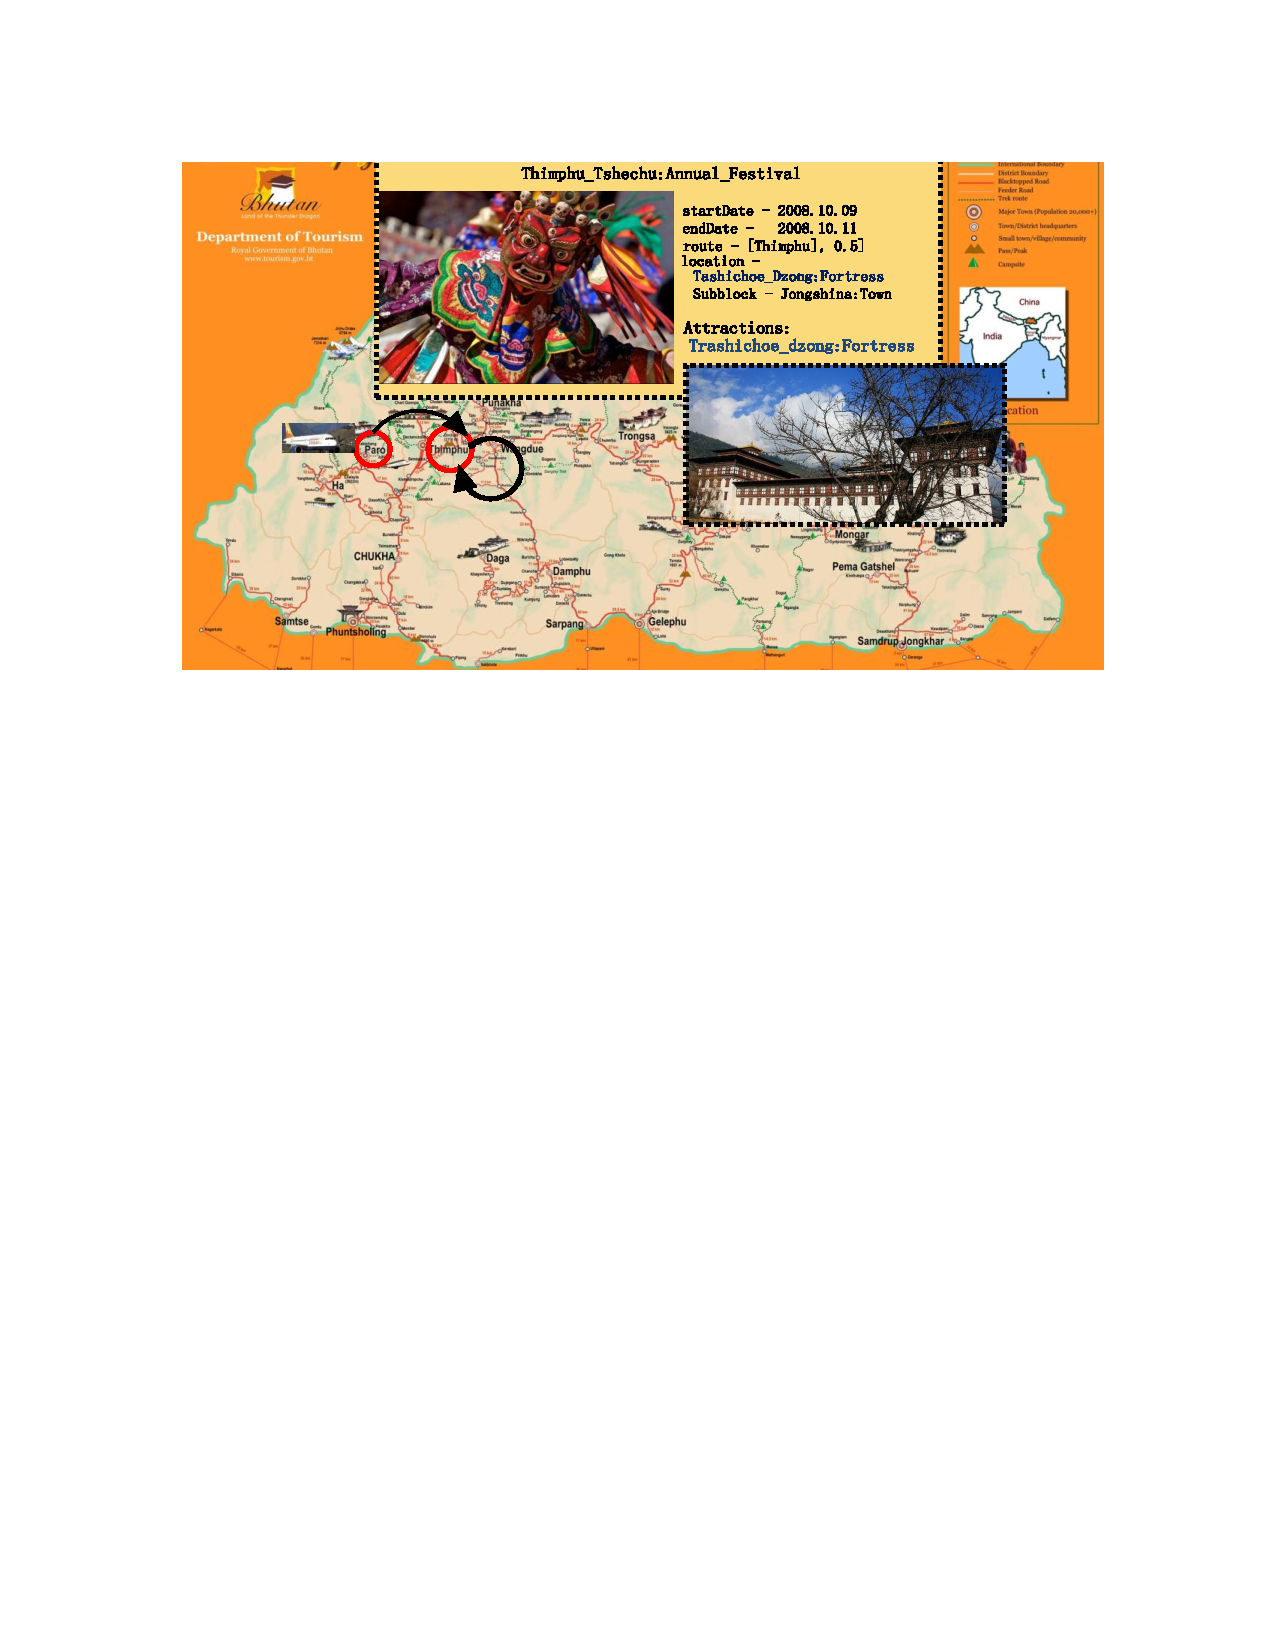
\includegraphics[width=11.5cm, height=7cm]{E3}
\caption{Travel Planning Scenario}
\end{figure}}
\frame{\frametitle{5.3.6 Travel Plan -Event 3 found}
\begin{figure}
\centering
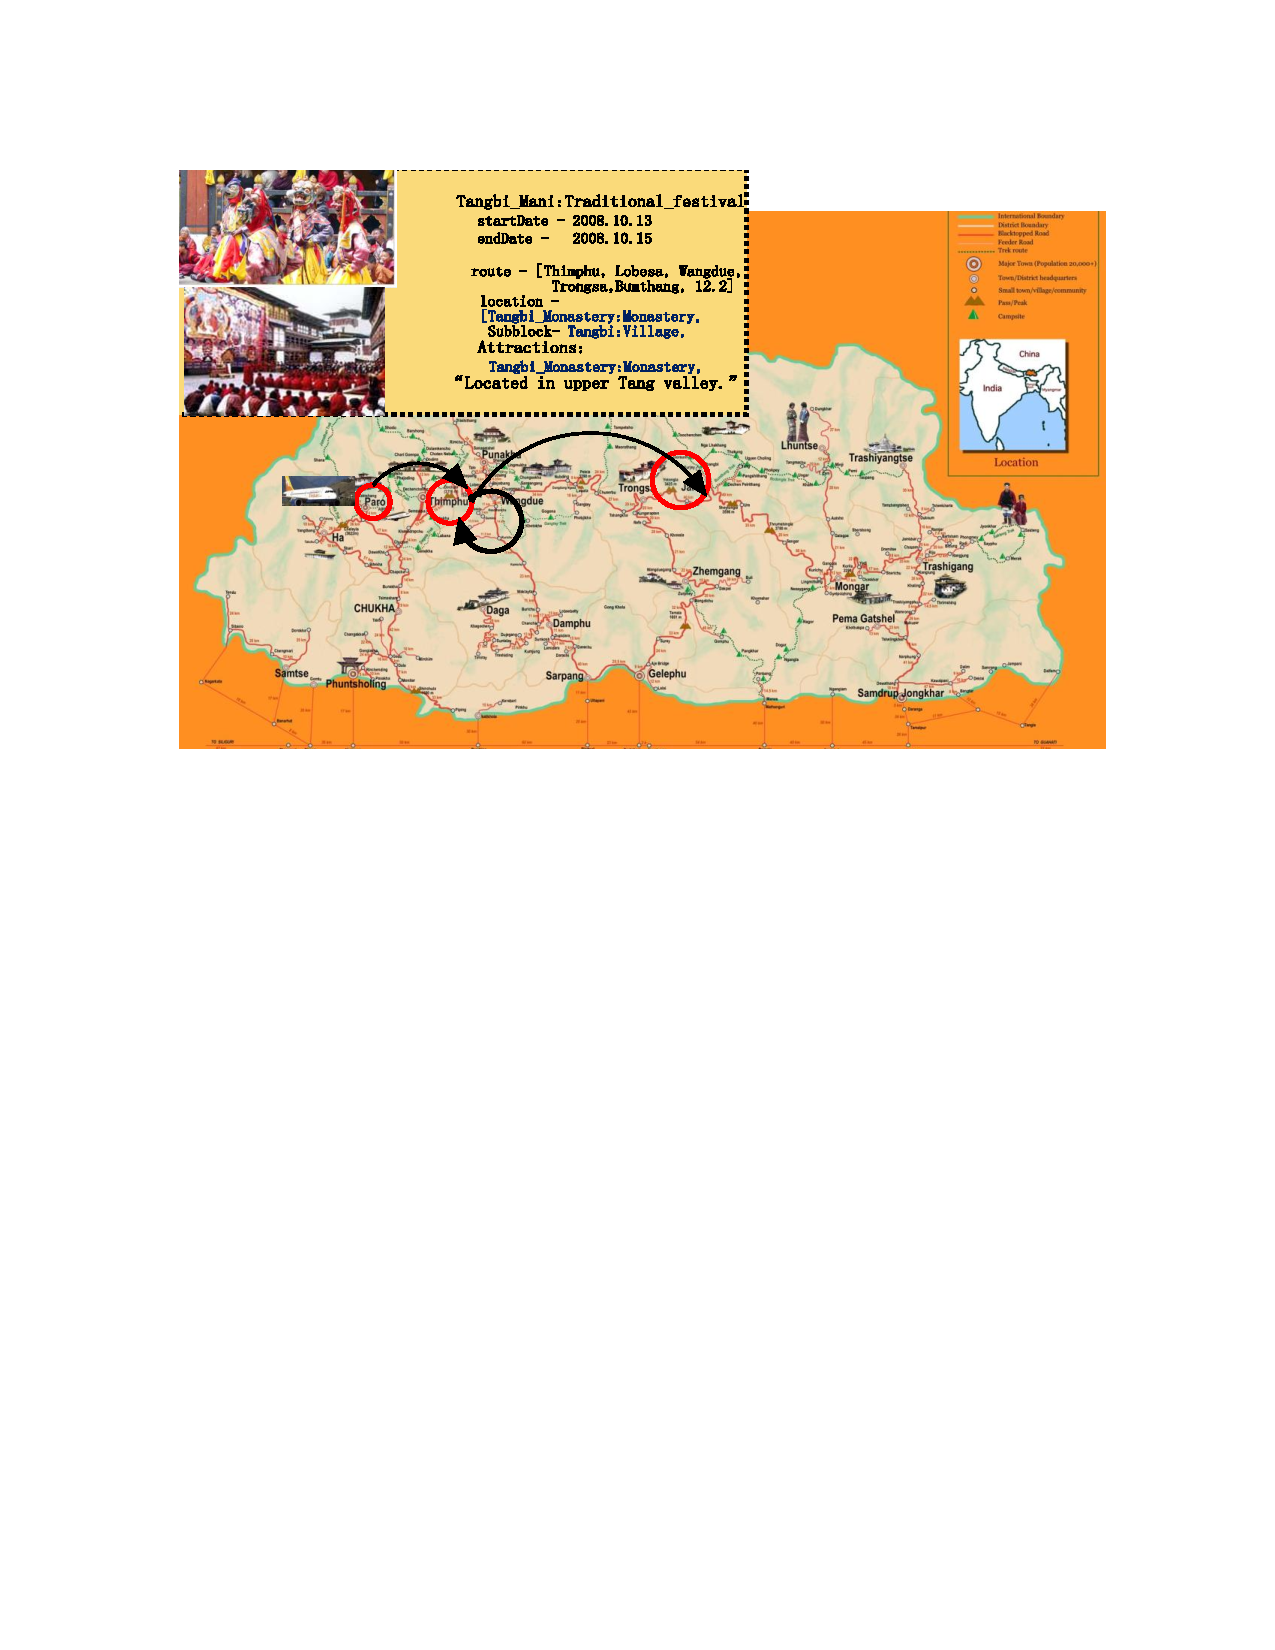
\includegraphics[width=11.5cm, height=7cm]{E4}
\caption{Travel Planning Scenario}
\end{figure}}
\frame{\frametitle{5.3.6 Travel Plan -Return route to the end point}
\begin{figure}
\centering
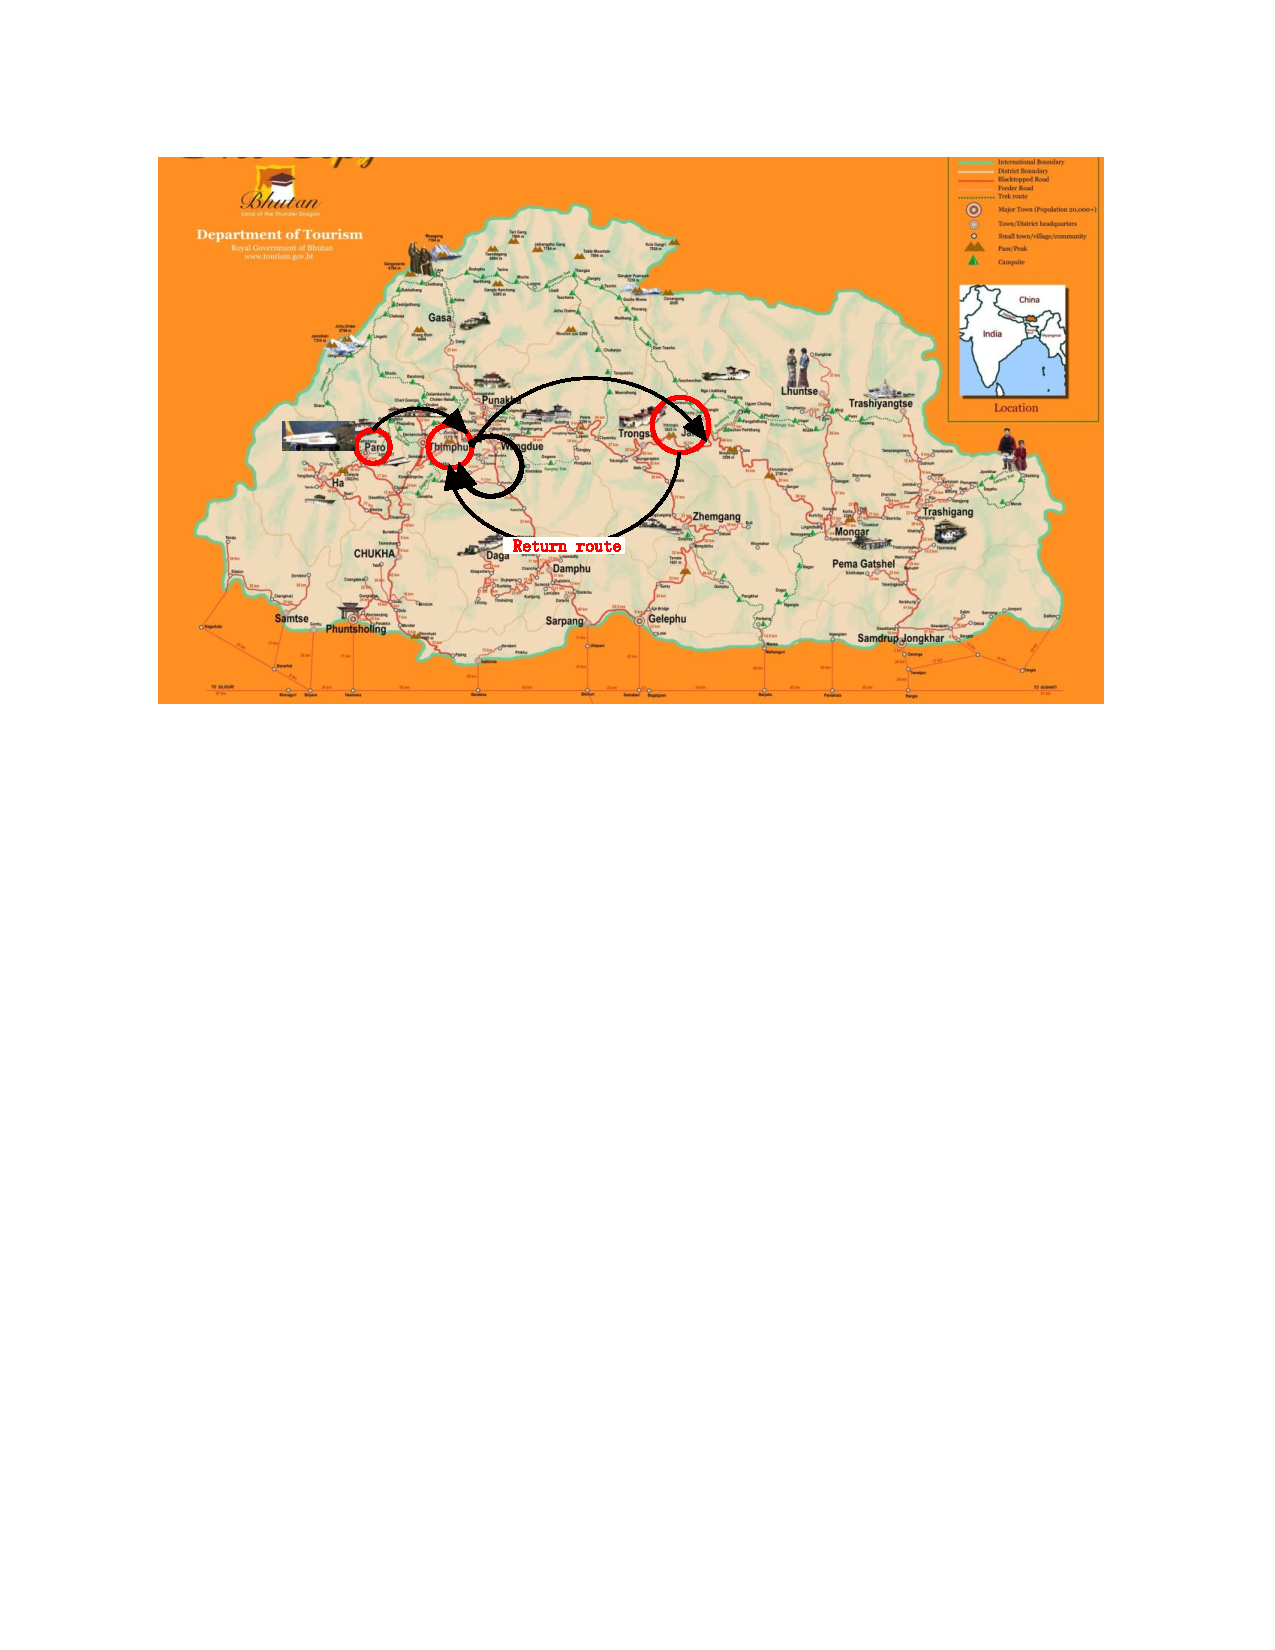
\includegraphics[width=11.5cm, height=7cm]{E5}
\caption{Travel Planning Scenario}
\end{figure}}

\frame{\frametitle{5.3.6 Travel Planning -On-route attraction recommendation (Optional)}
\begin{figure}
\centering
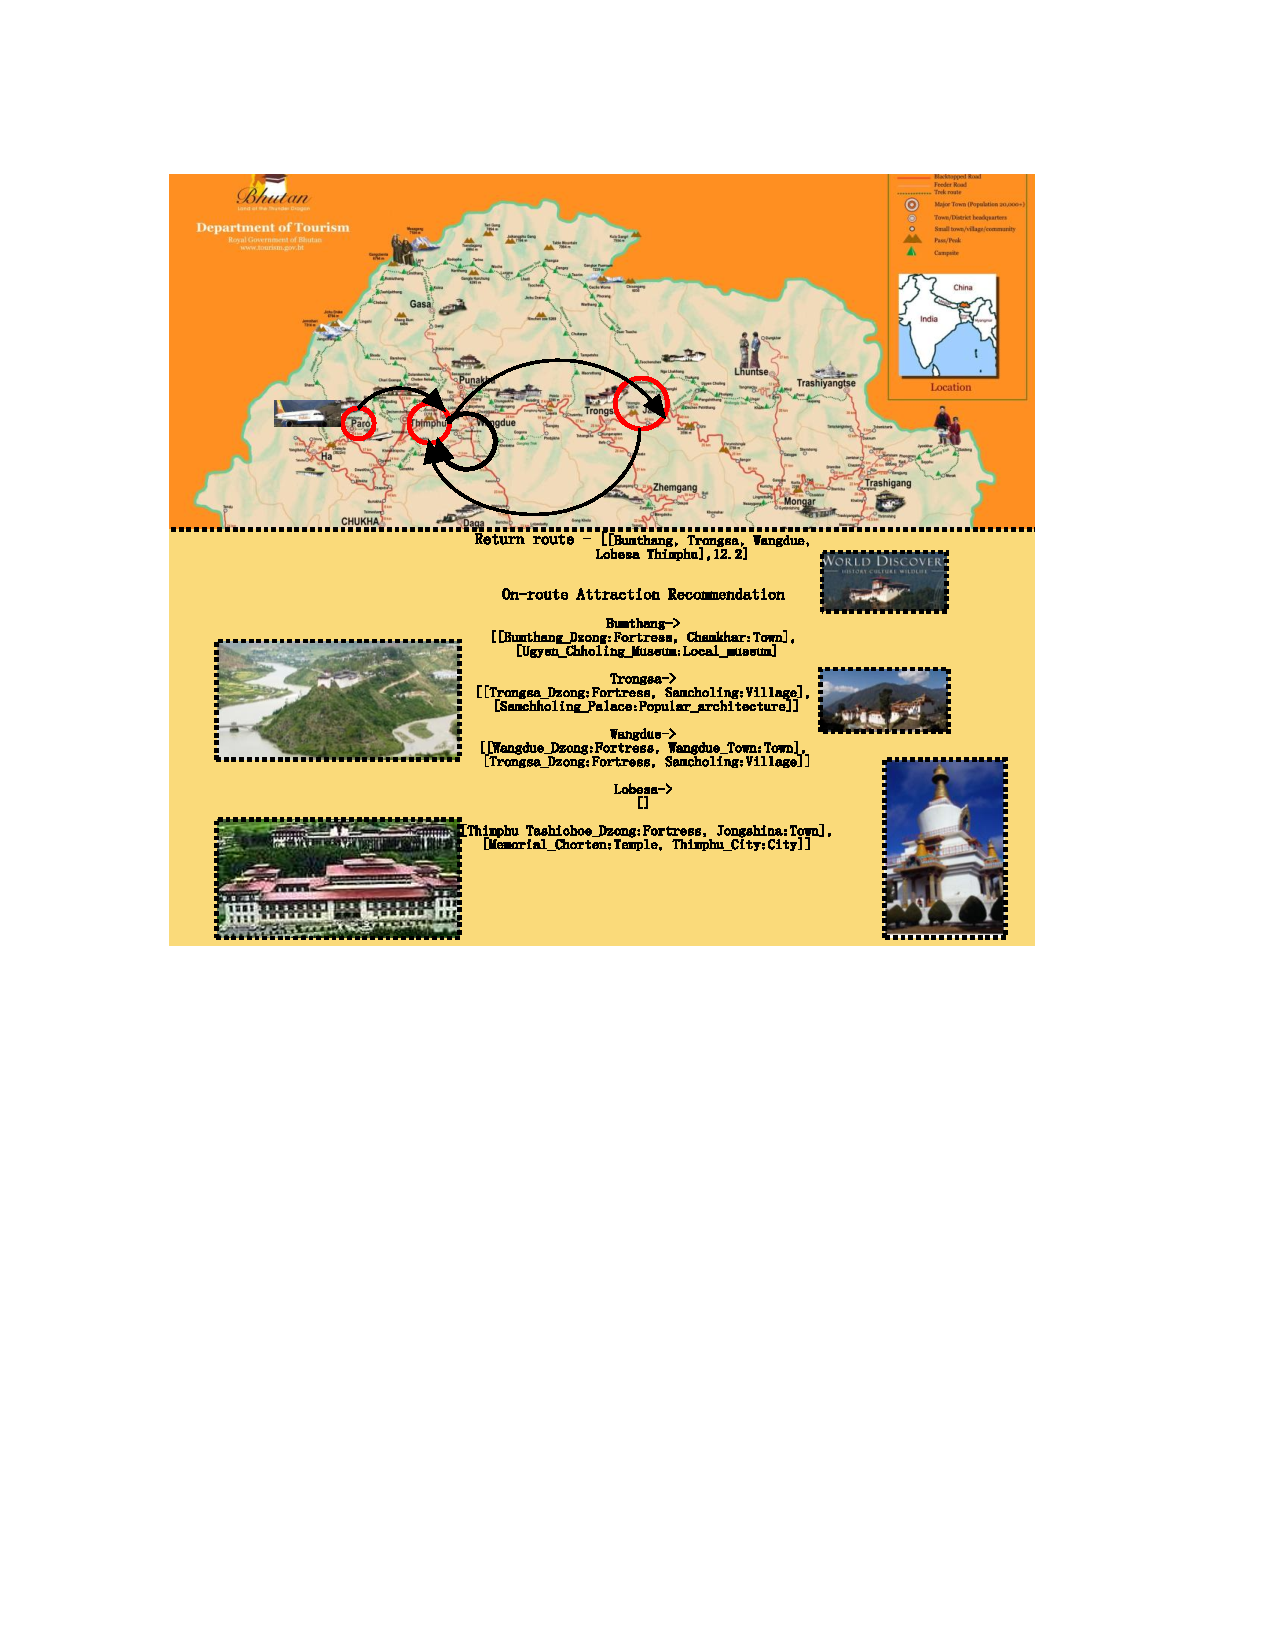
\includegraphics[width=11cm, height=7.5cm]{E6}
\caption{Travel Planning Scenario}
\end{figure}}


 
\frame{\frametitle{5.4.1 Execution times}
\begin{itemize}
\item \color{blue}Development \& Test environment:
\begin{itemize}
%\item Experiments performed in ITC 315
\item OO jDREW engine version 0.96
\item On Windows XP with Intel Core 2 Duo 2.66 GHz %processor
\end{itemize}
\end{itemize}

\begin{itemize}
\item \color{blue}eTourPlan KB:
\begin{itemize}
\item 115 classes, 73 facts, and 37 rules
\end{itemize}
\end{itemize}

\begin{itemize}
\item\color{blue}Low OO jDREW execution times for retrieving subdomain information:
\begin{itemize}
\item Object-centric profile descriptions for each of the subdomains are well-structured with {\color{blue}RDFS type definitions} and {\color{blue}partonomy rules}
\vspace{0.1in}
\item Search rules are {\color{blue}object-centric}; therefore search is {\color{blue}localised} to a specific domain
\end{itemize}
\end{itemize}
}
 
\frame{\frametitle{5.4.2 Execution times}

\begin{itemize}
\item\color{blue}High OO jDREW execution times for recursive search predicates:
\begin{itemize}
\vspace{0.2in}
\item Incorporation of recursive predicates such as ``getAllAttractions",
``getAllEvents", and ``getAllAccommodations"  \vspace{0.2in}
 %Another source of inefficiency is from 
\item The textual order between rules is not exploited by our pure logic programs (simulate exhaustive breadth-first parallel execution with iterative deepening)  %thereby performing unnecessary searches for candidate bindings. 
\vspace{0.2in}
\item For the recursive search predicates, execution times grow exponentially with the number of candidate activities
\end{itemize}
\end{itemize}
}
\section{6. Conclusion and Future Work}
%%%%%%%%%%%%%%%%%%%%%%%%%%%%%%%%%%%%%%%%%%
\subsection{6.1 Contributions}
\frame{\frametitle{6.1 Contributions}
\color{blue}\textbf{ eTourPlan: A knowledge-based tourist route and activity planner}
\pause
\begin{itemize}
\item \vspace{0.2cm} Designed and implemented a KB comprised of object-centric facts of Bhutan tourist information, structured by light weight ontologies
\pause
%\begin{itemize}
 %\item Profiles of 10 (of 20) touristic provinces of Bhutan and their tourist information
\item \vspace{0.2cm} Realized rule subsystems for various tourist services
 \begin{itemize}
 \item Semantic searches %to perform semantic searches of tourist entities
 \item Tour recommendation %for the administrative subdivision of a country
 \item Travel planning
 \end{itemize}
 \pause
 \item \vspace{0.2cm} Iterated through a step-wise "model and test" cycle to obtain the executable specification of the
eTourPlan prototype
 \pause
 \item \vspace{0.2in} Tested and evaluated the eTourPlan KB (115  classes, 73 facts, and 37 rules) in the
  OO jDREW reasoning engine:
  \begin{itemize}
% \item Explored the reasoning potentials of rules on a complete KB
\item \vspace{0.1cm}Constitutes a real world use case (based on Bhutan tourism information)
\item \vspace{0.1cm}Offers multiple options for a diversity of travel plans
\item \vspace{0.1cm}Provides precise parametric search results for various queries on the tourism KB
 \end{itemize}
\pause
 \item Demo can be given on demand
\end{itemize}
}


\frame{\frametitle{6.2 Future Work}
\begin{itemize}
% \pause  
\item \vspace{0.2cm} Other planning strategies such as partial planning and sequence planning
\item \vspace{0.2cm} Cost estimation for the total travel

\item \vspace{0.2cm} The current executable specification can be integrated with a database or
could be translated to a self-contained database application
\item \vspace{0.2cm} A user-friendly GUI would increase the utility of the key operations of
the eTourPlan prototype
\item \vspace{0.2in} The semantic model and search of eTourPlan can be extended to a ``Semantic Bhutan" portal
(and transferred to other regions such as New Brunswick)
\end{itemize}
}
\frame{\frametitle{Thank You}
\begin{figure}
\centering
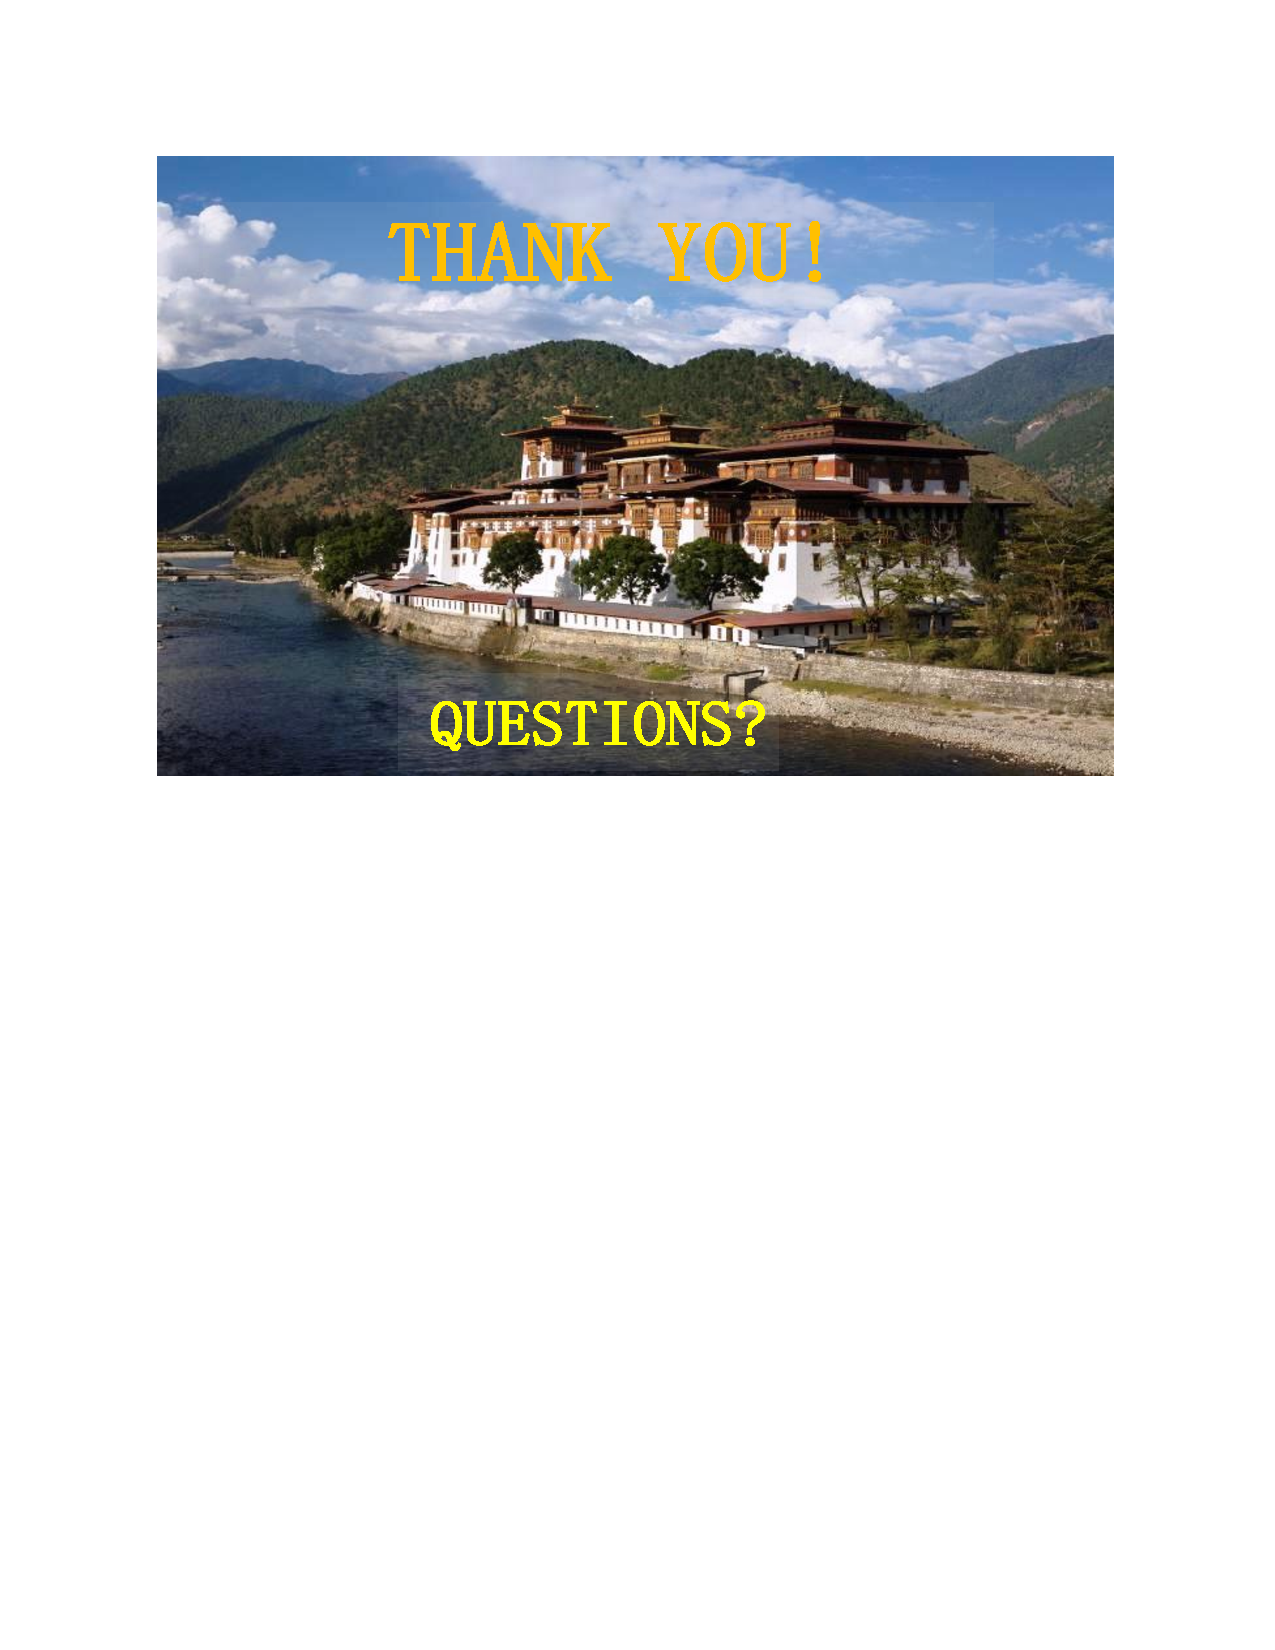
\includegraphics[width=11.5cm, height=7cm]{thanks.pdf}
\caption{Travel Planning Scenario}
\end{figure}}

\frame{\frametitle{}
\hspace{0.3in}\Huge \centering \textbf{ \color{blue}BACKUP SLIDES}\\
\vspace{0.2in}
}

%%%%%%%%%%%%%%%%%%%%%%%%%%%%%%%%%%%%%%%%%%%%%%%%%%%%%%%%%%%%%%%%%%%%%%%%%%
\section{more slides}
\frame{\frametitle{4.3.1.9 Search Rules}
\begin{figure} [tbph]
\centering
\footnotesize
\begin{tabular}{|l|}
\hline
\textbf{\color{blue}KB (Rules):}\\ 
\\
\color{blue}\%-----at a subblock level---------------------------------------------\%\\
 getAttraction(?Attraction:Attractions, ?Subblock:Subblock):-\\
 \hspace{0.1in}siteOf(?Attraction:Attractions, ?Subblock:Subblock).\\
   \\
 \color{blue}\%----at a block level-------------------------------------------------\%\\
 getAttraction(?Attraction:Attractions, ?Block:Block):-\\
  \hspace{0.1in}partOfBlock(?Attraction:Attractions, ?Block:Block).\\
  \\
 getAttraction(?Attraction:Attractions, ?Block:Block):-\\
   \hspace{0.1in}partOfBlock(?Subblock:Subblock, ?Block:Block),\\
   \hspace{0.1in}getAttraction(?Attraction:Attractions, ?Subblock:Subblock).\\
\\
 \color{blue}\%-----at a province level---------------------------------------------\%\\
 getAttraction(?Attraction:Attractions, ?Province:Province):-\\
   \hspace{0.1in}partOfProvince(?Attraction:Attractions, ?Province:Province).\\
 \\ 
 getAttraction(?Attraction:Attractions, ?Province:Province):-\\
   \hspace{0.1in}partOfProvince(?Block:Block, ?Province:Province),\\
   \hspace{0.1in}getAttraction(?Attraction:Attractions, ?Block:Block).\\
   
  \hline
\end{tabular}
\end{figure}
}

%%%%%%%%%%%%%%%%%%%%%%%%%%%%%%%%%%%%%%%%%%%%%%%%%%%%%%%%%%%%%%%%%%%%%%%%%%
\frame{\frametitle{4.3.1.10 Search Rules}
\begin{figure} [tbph]
\centering
\footnotesize
\begin{tabular}{|l|}
\hline
\textbf{\color{blue}KB:}\\ 
\\
\color{blue}\%-----at a region  level----------------------------------------------\%\\
 getAttraction(?Attraction:Attractions, ?Region:Region):-\\
   \hspace{0.1in}partOfRegion(?Attraction:Attractions, ?Region:Region).\\
 \\   
 getAttraction(?Attraction:Attractions, ?Region:Region):-\\
   \hspace{0.1in}partOfRegion(?Province:Province, ?Region:Region),\\
   \hspace{0.1in}getAttraction(?Attraction:Attractions, ?Province:Province).\\  
   
 \color{blue}\%----at a country level-----------------------------------------------\%\\

 getAttraction(?Attraction:Attractions, ?Country:Country):-\\
   \hspace{0.1in}partOfCountry(?Attraction:Attractions, ?Country:Country).\\

 getAttraction(?Attraction:Attractions, ?Country:Country):-\\
   \hspace{0.1in}partOfCountry(?Region:Region, ?Country:Country),\\
   \hspace{0.1in}getAttraction(?Attraction:Attractions, ?Region:Region).\\ 
  \\
 \textbf{\color{blue}Sample Queries:}\\
 \\
   getAttraction(?Attraction:Attractions, {\color{red}Bhutan:Country})\\
   getAttraction(?Attraction:Attractions, {\color{red}Western:Region})\\
   getAttraction(?Attraction:Attractions, {\color{red}Bumthang:Province})\\
   getAttraction(?Attraction:Attractions, {\color{red}Chhoekhor:Block})\\
   getAttraction(?Attraction:Attractions, {\color{red}Chamkhar:Town})\\
\hline
\end{tabular}
\end{figure}
}
\subsection{4.3.2 Distance Computation}
\frame{\frametitle{4.3.2.1 Route and Distance Time Computation}
\textbf{\color{blue}Facilitates the Transportation subdomain} \vspace{0.3cm}
\begin{itemize}
\item Two-level Computation
\begin{itemize}
\item Precomputation of all routes ({\color{blue} ``dTR" predicate})
\item Optimal route (i.e. shortest distance by {\color{blue} ``dTRShortest" predicate}) 
\end{itemize}
\vspace{0.2cm}
\item Implemented in the OO jDREW Top-Down FindAll Solutions architecture
\vspace{0.2cm}
\item Stored as precomputed facts in the KB
\end{itemize}
}

\frame{\frametitle{4.3.3 Precomputation of Route and Distance-time Facts}
\begin{figure}
\centering
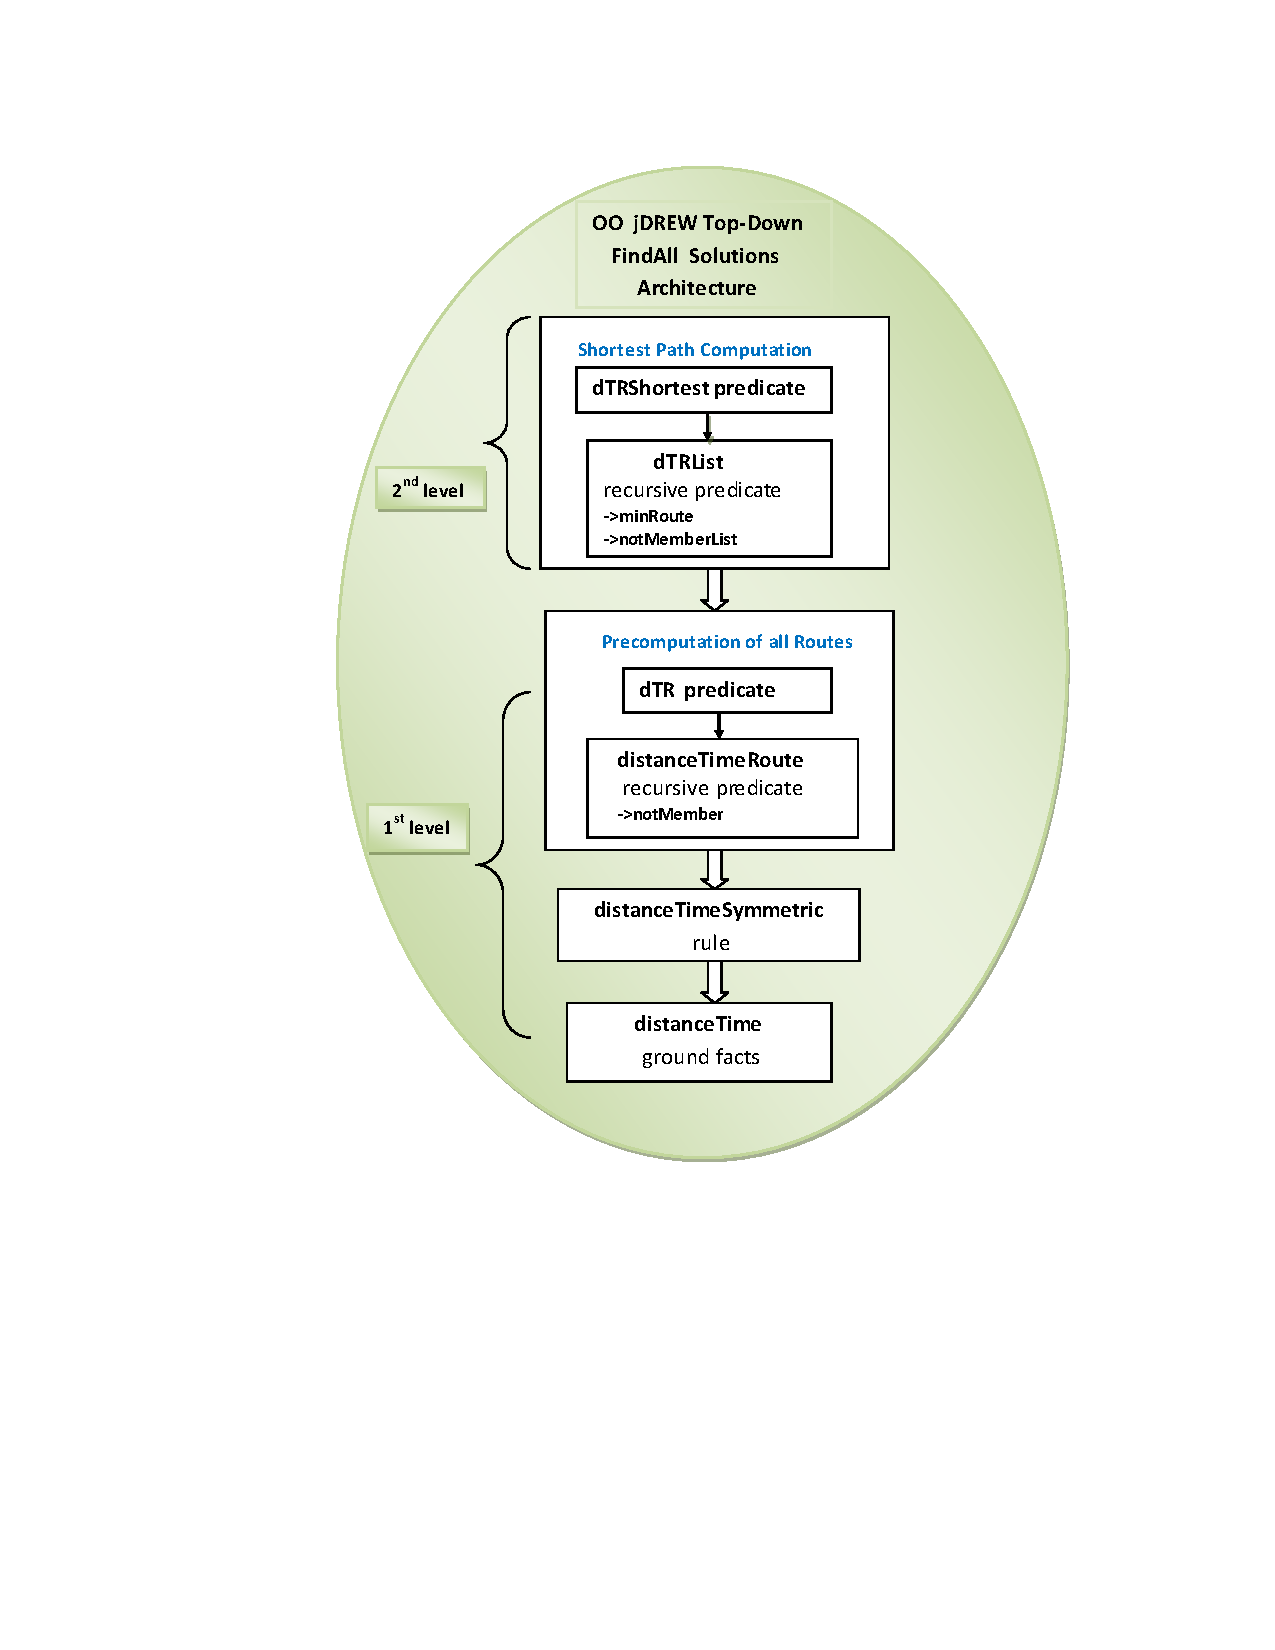
\includegraphics[width=6.5cm, height=7cm]{route.pdf}
\caption{Two-level Computation}
\end{figure}
}
%%%%%%%%%%%%%%%%%%%%%%%%%%%%%%%%%%%%%%%%%%%%%%%%%%%%%%%%%%%%%%%%%%%%%%%%%
%%%%%%%%%%%%%%%%%%%%%%%%%%%%%%%%%%%%%%%%%%%%%%%%%%%%%%%%%%%%%%%%%%%%%%%%%%
\frame{\frametitle{4.3.1.6 Partonomy Extensions (Sample KB)}
\begin{figure} [tbph]
\centering
\begin{itemize}
\item \textbf{\color{blue}``getFullAddress" Rule extended}
\begin{itemize}
\item Computes a location based on GPS coordinates
\item Precise addressing scheme
\end{itemize}
\end{itemize}
\\
\vspace{0.2in}
\footnotesize
\begin{tabular}{|l|}
\hline
\textbf{\color{blue}Sample GPS Facts:}\\
\\
 address(Bumthang\_Dzong:Fortress, \\
  \hspace{0.3in}Loc[latitude-$>$Detail[degree-$>$48:Real; minute-$>$0:Real];\\
  \hspace{0.45in}   longitude-$>$Detail[degree-$>$66:Real; minute-$>$40:Real]]).\\
\textbf{\color{blue}Rule:}\\ 
\\
getFullAddress(?Location, [?Subblock, ?Block, ?Province, ?Region, ?Country, \\
\hspace{0.65in}             ?Latitude, ?Longitude]):-\\
\hspace{0.1in} \color{red}   getLatitude(?Location, ?Latitude),\\
 \hspace{0.1in} \color{red}  getLongitude(?Location, ?Longitude),\\
 \hspace{0.1in}   siteOf(?Location, ?Subblock),\\
 \hspace{0.1in}   partOfBlock(?Subblock, ?Block),\\
 \hspace{0.1in}   partOfProvince(?Block, ?Province),\\
 \hspace{0.1in}   partOfRegion(?Province, ?Region),\\
 \hspace{0.1in}   partOfCountry(?Region, ?Country).\\
 \hline
\end{tabular}
\end{figure}
}


%%%%%%%%%%%%%%%%%%%%%%%%%%%%%%%%%%%%%%%%%%%%%%%%%%%%%%%%%%%%%%%%%%%%%%%%%%
\frame{\frametitle{4.3.1.7 Partonomy KB (Query and Result)}
\begin{figure} [tbph]
\centering
\footnotesize
\begin{tabular}{|l|}
\hline
\textbf{\color{blue}Sample Query:} \\ 
\\
 getFullAddress(Bumthang\_Dzong:Fortress, ?Address)\\
 \\
 \textbf{\color{blue}OO jDREW TD Result:}\\
 \\
  ?Address= [\color{red}4800.0:Real,\\
   \hspace{0.5in}\color{red}6666.666666666667:Real,\\
   \hspace{0.5in}Chamkhar:Town,\\
   \hspace{0.5in}Chhoekhor:Block,\\
   \hspace{0.5in}Bumthang:Province,\\
   \hspace{0.5in}Central:Region,\\
   \hspace{0.5in}Bhutan:Country]\\
\hline
\end{tabular}
\end{figure}
}


\frame{\frametitle{5.1.2 Sample Search Queries}
\begin{table} [tbph]
%\caption{Activity search result of Query 4}
\centering
\footnotesize
\begin{tabular}{|l|l|l|}
\hline
 Query&\textbf{Entity} &$~~~~~~~~~~~~~~~~~~~~~~~~~~$\textbf{Search Query} \\
\hline
 1&Province & getProvinceDetails(region-$>?$Region:Region;\\
  &        &$~~~~~~~~~~~~~~~~~~~~~~~~~~~~~~~~$name-$>$\textbf{{\color{blue}Bumthang}:Province}; \\
  &        &$~~~~~~~~~~~~~~~~~~~~~~~~~~~~~~~${\color{red}$?$ProvinceDetails})\\
 \hline
 2&Route &getRouteDetails(startPoint-$>$\textbf{{\color{blue}Chukha}:Province};\\
  &   &$~~~~~~~~~~~~~~~~~~~~~~~~~~$endPoint-$>$\textbf{{\color{blue}Punakha}:Province}; \\
  &       &$~~~~~~~~~~~~~~~~~~~~~~~~~~${\color{red}$?$RouteDetails},\\
  &       &$~~~~~~~~~~~~~~~~~~~~~~~~~~${\color{red}$?$ShortestRoute})\\  
 \hline
  3&Activity & getActivityDetails(actName-$>?$Name:\textbf{{\color{blue}Events}};\\
  &&$~~~~~~~~~~~~~~~~~~~~~~~~~~~~~~$theme-$>$\textbf{{\color{blue}Recreation}}; \\
  &       &$~~~~~~~~~~~~~~~~~~~~~~~~~~~~~~$address-$>$[?Subblock, \\
  &                       &$~~~~~~~~~~~~~~~~~~~~~~~~~~~~~~~~~~~~~~~~~~~~~~~?$Block, \\
  &                       &$~~~~~~~~~~~~~~~~~~~~~~~~~~~~~~~~~~~~~~~~~~~~~~~?$Province,\\
  &                       &$~~~~~~~~~~~~~~~~~~~~~~~~~~~~~~~~~~~~~~~~~~~~~~$\textbf{{\color{blue}Southern:Region}}, \\
  &                       &$~~~~~~~~~~~~~~~~~~~~~~~~~~~~~~~~~~~~~~~~~~~~~~~?$Country]; \\
  &                 &$~~~~~~~~~~~~~~~~~~~~~~~~~~~~~${\color{red}$?$ActivityDetails})\\ 
  \hline
   4& Accommodation & getAccommodationDetails(accName-$>?$Name:\textbf{{\color{blue}Resort}};\\
  & &$~~~~~~~~~~~~~~~~~~~~~~~~~~~~~~~~~~~~~~~~~~~$address-$>$[\textbf{{\color{blue}Tsento\_Shari:Village}}, \\
  &     &$~~~~~~~~~~~~~~~~~~~~~~~~~~~~~~~~~~~~~~~~~~~~~~~~~~~~~~~~~~~~?$Block, \\
  &                    &$~~~~~~~~~~~~~~~~~~~~~~~~~~~~~~~~~~~~~~~~~~~~~~~~~~~~~~~~~~~~?$Province,  \\
  &                    &$~~~~~~~~~~~~~~~~~~~~~~~~~~~~~~~~~~~~~~~~~~~~~~~~~~~~~~~~~~~~?$Region, \\
  &                    &$~~~~~~~~~~~~~~~~~~~~~~~~~~~~~~~~~~~~~~~~~~~~~~~~~~~~~~~~~~~~?$Country]; \\ 
  &                    &$~~~~~~~~~~~~~~~~~~~~~~~~~~~~~~~~~~~~~~~~~~~$setMaxPrice-$>$[\textbf{{\color{blue}Yes}},\\
  &              &$~~~~~~~~~~~~~~~~~~~~~~~~~~~~~~~~~~~~~~~~~~~~~~~~~~~~~~~~~~~~~~~~~~~~$\textbf{{\color{blue}1500}}:Real]; \\ 
  &                    &$~~~~~~~~~~~~~~~~~~~~~~~~~~~~~~~~~~~~~~~~~~${\color{red}$?$AccommodationDetails})\\
\hline
 \end{tabular} 
\end{table}}
}


\frame{\frametitle{5.1.1 Search for Provincial Information \normalsize(Input Modes and Search Result for Query 1)}
\begin{table} [tbph]
%\caption{Queries of different input/output for Province search}
\centering
\footnotesize
\begin{tabular}{|l|l|l|}
\hline
 Query&\textbf{User Input} &$~~~~~~~~~~~~~~~~~~~~$ \textbf{Query Formats} \\
 &$~~$\textbf{Values}   &$~~~~~~~~~~~~$(Input values are bold-faced)     \\
\hline
 1&name & getProvinceDetails(region-$>?$Region:Region;\\
  &        &$~~~~~~~~~~~~~~~~~~~~~~~~~~~~~~~~$name-$>$\textbf{{\color{blue}Bumthang}:Province}; \\
  &       &$~~~~~~~~~~~~~~~~~~~~~~~~~~~~~~~${\color{red}$?$ProvinceDetails})\\
          
 \hline
 2&region & getProvinceDetails(region-$>$\textbf{{\color{blue}Central}:Region};\\
  &        &$~~~~~~~~~~~~~~~~~~~~~~~~~~~~~~~~$name-$>$?Name:Province; \\
  &        &$~~~~~~~~~~~~~~~~~~~~~~~~~~~~~~~${\color{red}$?$ProvinceDetails})\\
 \hline
 3&None & getProvinceDetails(region-$>?$Region:Region;\\
  &        &$~~~~~~~~~~~~~~~~~~~~~~~~~~~~~~~~$name-$>$?Name:Province; \\
  &        &$~~~~~~~~~~~~~~~~~~~~~~~~~~~~~~~${\color{red}$?$ProvinceDetails})\\         
\hline
\end{tabular} 
\end{table}
\footnotesize
\pause 
\begin{table} [tbph]
%\caption{Province search result of Query 1}
\centering
\begin{tabular}{|l|l|}
\hline
 \textbf{Output} &$~~~~~~~~~~~~~~~~~~~~~~~~~~$\textbf{Variable Bindings} \\
 \textbf{Variables}&$~~~~~~~~~~~~~~~~~~~~~~~~~~~~~~$(For Query 1)            \\
\hline
 {\color{red}$?$ProvinceDetails}&[WebLink-$>$``http://www.bumthang.gov.bt/";\\
          &$~$Description-$>$``Bumthang is one of the most attractive touristic  \\
        &$~~~~~~~~~~~~~~~~~~~~~~~~~$province with several festivals throughout the year";\\
        &$~$Capital-$>$Chamkhar:Town; \\
        &$~$Geography-$>$[Area-$>$"1,819 sq.km";\\
        &$~~~~~~~~~~~~~~~~~~~~~~$Elevation-$>$"1,300 to 7300 meters"];\\
        &$~$TouristInfo-$>$[NumAttractions-$>$16:Integer;\\ 
           &$~~~~~~~~~~~~~~~~~~~~~~$NumEvents-$>$13:Integer; \\
				   &$~~~~~~~~~~~~~~~~~~~~~~$NumAccommodations-$>$10 :Integer]; \\
	      &$~$Contact-$>$"admbumthang@druknet.bt"] \\
 \hline
 {\color{red}$?$Region:Region}&Central:Region\\
\hline
\end{tabular} 
\end{table}
}

\frame{\frametitle{5.1.2 Search for Route Details \normalsize(Input/Output Modes)}
\begin{table} [tbph]
%\caption{Query mode (input/output) for Route search}
\centering
\footnotesize
\begin{tabular}{|l|l|l|}
\hline
Query &\textbf{User Input} &$~~~~~~~~~~~~~~~~~~~~$ \textbf{Query Formats} \\
 &$~~$\textbf{Values}   & $~~~~~~~~~~~~$(Input values are bold-faced)      \\
\hline
 1&startPoint &getRouteDetails(startPoint-$>$\textbf{{\color{blue}Chukha}:Province};\\
  &endPoint   &$~~~~~~~~~~~~~~~~~~~~~~~~~~$endPoint-$>$\textbf{{\color{blue}Punakha}:Province}; \\
  &       &$~~~~~~~~~~~~~~~~~~~~~~~~~~${\color{red}$?$RouteDetails},\\
  &       &$~~~~~~~~~~~~~~~~~~~~~~~~~~${\color{red}$?$ShortestRoute})\\  
\hline
\end{tabular} 
\end{table}

\pause \begin{table} [tbph]
%\caption{Route search result for Query 1}
\centering
\footnotesize
\begin{tabular}{|l|l|}
\hline
 \textbf{Output} &$~~~~~~~~~~~~~~~~~~~~~~~~~~$\textbf{Variable Bindings} \\
 \textbf{Variables}&$~~~~~~~~~~~~~~~~~~~~~~~~~~~~~~$(For Query 1)         \\
\hline
{\color{red}$?$RouteDetails}&[[[[Chukha, Chuzom, Thimphu, Lobesa, Punakha],\\
                &$~~~$11.2:Real], \\          
                &[[Chukha, Chuzom, Thimphu, Lobesa, WangduePhodrang, Punakha],\\
                &$~~~$11.90:Real]];\\
                &numRoutes-$>$2:Integer] \\
 \hline
{\color{red} $?$ShortestRoute}& [[[Chukha, Chuzom, Thimphu, Lobesa, Punakha], \\
                 &$~~~$11.2 : Real]\\
\hline
\end{tabular} 
\end{table}
}


\frame{\frametitle{5.1.3 Search for Activity Oppurtunities (Input/Output Modes)}
\begin{table} [tbph]
%\caption{Queries of different input/output for Activity search}
\centering
\tiny
\begin{tabular}{|l|l|l|}
\hline
Query &\textbf{User Input} &$~~~~~~~~~~~~~~~~~~~~$ \textbf{Query Formats} \\
 &$~~$\textbf{Values}   & $~~~~~~~~~~~~$(Input values are bold-faced)      \\
\hline
 1&$~~$actName & getActivityDetails(actName-$>$\textbf{{\color{blue}Paro\_Tshechu:Events}};\\
  &        &$~~~~~~~~~~~~~~~~~~~~~~~~~~~~~$theme-$>?$Theme; \\
  &        &$~~~~~~~~~~~~~~~~~~~~~~~~~~~~~$address-$>?$Address; \\
  &        &$~~~~~~~~~~~~~~~~~~~~~~~~~~~~${\color{red}$?$ActivityDetails})\\
          
\hline
 2&$~~$actName:\emph{type} & getActivityDetails(actName-$>?$Name:\textbf{{\color{blue}Festivals}};\\
  &$~~~~$and/or      &$~~~~~~~~~~~~~~~~~~~~~~~~~~~~~$theme-$>?$Theme; \\
  & address element     &$~~~~~~~~~~~~~~~~~~~~~~~~~~~~~$address-$>$[?Subblock, \\
  &                       &$~~~~~~~~~~~~~~~~~~~~~~~~~~~~~~~~~~~~~~~~~~~~~~$\textbf{{\color{blue}Chhoekhor:Block}}, \\
  &                       &$~~~~~~~~~~~~~~~~~~~~~~~~~~~~~~~~~~~~~~~~~~~~~~~?$Province,  \\
  &                       &$~~~~~~~~~~~~~~~~~~~~~~~~~~~~~~~~~~~~~~~~~~~~~~~?$Region, \\
  &                       &$~~~~~~~~~~~~~~~~~~~~~~~~~~~~~~~~~~~~~~~~~~~~~~~?$Country]; \\
  &                 &$~~~~~~~~~~~~~~~~~~~~~~~~~~~~~${\color{red}$?$ActivityDetails})\\
          
\hline
 3&$~~~$theme & getActivityDetails(actName-$>?$Name;\\
  &$~~~~$and/or      &$~~~~~~~~~~~~~~~~~~~~~~~~~~~~~~$theme-$>$\textbf{{\color{blue}Cultural\_Religious\_Heritage}}; \\
  & address element      &$~~~~~~~~~~~~~~~~~~~~~~~~~~~~~~$address-$>$[?Subblock, \\
  &                       &$~~~~~~~~~~~~~~~~~~~~~~~~~~~~~~~~~~~~~~~~~~~~~~~~?$Block, \\
  &                       &$~~~~~~~~~~~~~~~~~~~~~~~~~~~~~~~~~~~~~~~~~~~~~~~$\textbf{{\color{blue}Paro:Province}},\\
  &                       &$~~~~~~~~~~~~~~~~~~~~~~~~~~~~~~~~~~~~~~~~~~~~~~~~?$Region, \\
  &                       &$~~~~~~~~~~~~~~~~~~~~~~~~~~~~~~~~~~~~~~~~~~~~~~~~?$Country]; \\
  &                 &$~~~~~~~~~~~~~~~~~~~~~~~~~~~~${\color{red}$?$ActivityDetails})\\          
\hline 
 4&$~~~~$theme & getActivityDetails(actName-$>?$Name:\textbf{{\color{blue}Events}};\\
  &$~~~~$actName:\emph{type}&$~~~~~~~~~~~~~~~~~~~~~~~~~~~~~~$theme-$>$\textbf{{\color{blue}Recreation}}; \\
  & address element      &$~~~~~~~~~~~~~~~~~~~~~~~~~~~~~~$address-$>$[?Subblock, \\
  &                       &$~~~~~~~~~~~~~~~~~~~~~~~~~~~~~~~~~~~~~~~~~~~~~~~?$Block, \\
  &                       &$~~~~~~~~~~~~~~~~~~~~~~~~~~~~~~~~~~~~~~~~~~~~~~~?$Province,\\
  &                       &$~~~~~~~~~~~~~~~~~~~~~~~~~~~~~~~~~~~~~~~~~~~~~~$\textbf{{\color{blue}Southern:Region}}, \\
  &                       &$~~~~~~~~~~~~~~~~~~~~~~~~~~~~~~~~~~~~~~~~~~~~~~~?$Country]; \\
  &                 &$~~~~~~~~~~~~~~~~~~~~~~~~~~~~~${\color{red}$?$ActivityDetails})\\        
 \hline
 5&$~~~~$None              & getActivityDetails(actName-$>?$Name;\\
  &    &$~~~~~~~~~~~~~~~~~~~~~~~~~~~~~$theme-$>$Theme; \\
  &       &$~~~~~~~~~~~~~~~~~~~~~~~~~~~~~$address-$>?$Address; \\
  &      &$~~~~~~~~~~~~~~~~~~~~~~~~~~~~~~${\color{red}$?$ActivityDetails})\\ 
\hline 
\end{tabular} 
\end{table}
}

\frame{\frametitle{5.1.4  Activity Search Result of Query 4}
\begin{table} [tbph]
%\caption{Activity search result of Query 4}
\centering
\footnotesize
\begin{tabular}{|l|l|}
\hline
 \textbf{Output} &$~~~~~~~~~~~~~~~~~~~~~~~~~~$\textbf{Variable Bindings} \\
 \textbf{Variables}& $~~~~~~~~~~~~~~~~~~~~~~~~~~~~~~$(For Query 4)\\
\hline
 {\color{red}$?$ActivityDetails}&[ActName-$>$Yangphel\_Archery\_Tournament:Sport\_archery;\\
           &$~$WebLink-$>$``http://www.bhutanarchery.com/default.asp"; \\
		   &$~$EventDates-$>$[StartDate-$>$date[2008:Real, 08:Real, 23:Real];\\
           &$~~~~~~~~~~~~~~~~~~~~~~~~$EndDate-$>$date[2008:Real, 10:Real, 02:Real]];\\	   
          &$~$Description-$>$``11TH Yangphel open archery tournament";\\
          &$~$Address-$>$[Phuentsholing\_Upper\_Town:Town, \\
		&$~~~~~~~~~~~~~~~~~~~$Phuentsholing:Block, \\
		&$~~~~~~~~~~~~~~~~~~~$Chukha:Province, \\
		&$~~~~~~~~~~~~~~~~~~~$Southern:Region,\\
        &$~~~~~~~~~~~~~~~~~~~$Bhutan:Country];\\
		&$~$Theme-$>$Recreation;\\
        &$~$RelatedTo-$>$``Thimphu\_Drupchen:Annual\_festival"] \\
\hline
\end{tabular} 
\end{table}}

%%%%%%%%%%%%%%%%%%%%%%%%%%%%%%%%%%%%%%%%%%%%%%%%%%%%%%%%%%%%%%%%%%%%%%%%%%
\frame{\frametitle{3.3.6 Accommodations Class}
\begin{figure}[h] 
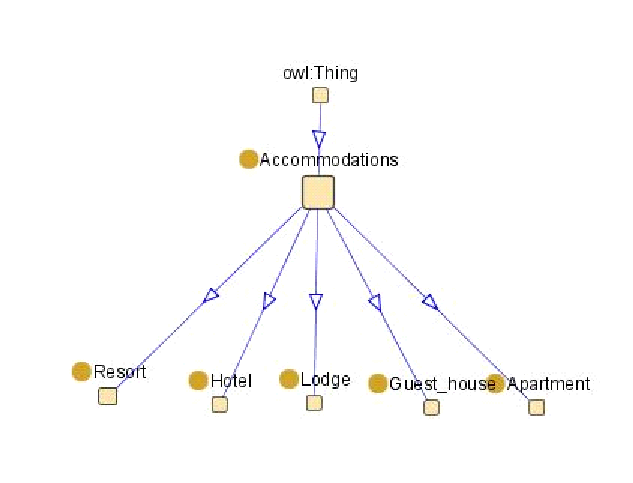
\includegraphics[width=7cm, height=3cm]{AccommodationClass}
\end{figure}

\begin{figure} [tbph]
\centering
\footnotesize
\begin{tabular}{|l|}
\hline
---------------------------------------------\\
\textbf{\color{blue}Profile of Wangdicholing\_Lodge}\\
---------------------------------------------\\   
      \textbf{accommodation}({\color{red}Wangdicholing\_Lodge:Lodge}$^{\wedge}$\\
      \hspace{0.95in}        {\color{blue}hs.url}->``http://www.wangdicholing.bt/'';\\
      \hspace{0.95in}        {\color{blue}et.rating}->3:Real;\\
      \hspace{0.95in}        {\color{blue}et.minPrice}->800:Real;\\
      \hspace{0.95in}        {\color{blue}et.subblock}->Chamkhar:Town;\\
      \hspace{0.95in}       {\color{blue}et.province}->Bumthang:Province;\\
      \hspace{0.95in}        {\color{blue}hs.telecoms}->Telecoms[\\
      \hspace{1.9in}               {\color{blue}et.landline}->9753631452;\\
       \hspace{1.9in}               {\color{blue}et.cell}->97517682948];\\
       \hspace{0.95in}      {\color{blue}hs.contact}->``manager@wangdicholing.bt'';\\
       \hspace{0.95in}      {\color{blue}\large{\textbf{hs.relatedTo}}}->{\color{red}Yangphel\_Guest\_house:Guest\_house}). \\  
\hline
\end{tabular}
\end{figure}
}

\frame{\frametitle{5.1.5 Search for Accommodation Details}
\begin{table} [tbph]
%\caption{Queries of different input/output for Accommodation search}
\centering
\tiny
\begin{tabular}{|l|l|l|}
\hline
 Query&\textbf{User Input} &$~~~~~~~~~~~~~~~~~~~~$ \textbf{Query Formats} \\
 &$~~$\textbf{Values}   &  $~~~~~~~~~~~~$(Input values are bold-faced)       \\
\hline
 1&$~~$accName & getAccommodationDetails(accName-$>$\textbf{{\color{blue}Aman\_Resort:Resort}};\\
  &        &$~~~~~~~~~~~~~~~~~~~~~~~~~~~~~~~~~~~~~~~~~~~$address-$>?$Address; \\
  &        &$~~~~~~~~~~~~~~~~~~~~~~~~~~~~~~~~~~~~~~~~~~~$setMaxPrice-$>?$SetMaxPrice; \\
  &        &$~~~~~~~~~~~~~~~~~~~~~~~~~~~~~~~~~~~~~~~~~~${\color{red}$?$AccommodationDetails})\\
\hline
 2&$~~$accName:\emph{type} & getAccommodationDetails(accName-$>?$Name:\textbf{{\color{blue}Guest\_house}};\\
  &$~~~~$and/or      &$~~~~~~~~~~~~~~~~~~~~~~~~~~~~~~~~~~~~~~~~~~~$address-$>$[\textbf{{\color{blue}Chamkhar:Town}}, \\
  &address element  &$~~~~~~~~~~~~~~~~~~~~~~~~~~~~~~~~~~~~~~~~~~~~~~~~~~~~~~~~~~~~?$Block, \\
  &                       &$~~~~~~~~~~~~~~~~~~~~~~~~~~~~~~~~~~~~~~~~~~~~~~~~~~~~~~~~~~~~?$Province,  \\
  &                       &$~~~~~~~~~~~~~~~~~~~~~~~~~~~~~~~~~~~~~~~~~~~~~~~~~~~~~~~~~~~~?$Region, \\
  &                       &$~~~~~~~~~~~~~~~~~~~~~~~~~~~~~~~~~~~~~~~~~~~~~~~~~~~~~~~~~~~~?$Country]; \\ 
  &                       &$~~~~~~~~~~~~~~~~~~~~~~~~~~~~~~~~~~~~~~~~~~~$setMaxPrice-$>?$SetMaxPrice;\\                
  &                        &$~~~~~~~~~~~~~~~~~~~~~~~~~~~~~~~~~~~~~~~~~~${\color{red}$?$AccommodationDetails})\\      
\hline
 3&$~~$setMaxPrice & getAccommodationDetails(accName-$>?$Name;\\
  &$~~~~$and/or      &$~~~~~~~~~~~~~~~~~~~~~~~~~~~~~~~~~~~~~~~~~~~$address-$>$[\textbf{{\color{blue}Chamkhar:Town}}, \\
  &address element   &$~~~~~~~~~~~~~~~~~~~~~~~~~~~~~~~~~~~~~~~~~~~~~~~~~~~~~~~~~~~~?$Block, \\
  &                   &$~~~~~~~~~~~~~~~~~~~~~~~~~~~~~~~~~~~~~~~~~~~~~~~~~~~~~~~~~~~~?$Province,  \\
  &                   &$~~~~~~~~~~~~~~~~~~~~~~~~~~~~~~~~~~~~~~~~~~~~~~~~~~~~~~~~~~~~?$Region, \\
  &                   &$~~~~~~~~~~~~~~~~~~~~~~~~~~~~~~~~~~~~~~~~~~~~~~~~~~~~~~~~~~~~?$Country]; \\ 
  &               &$~~~~~~~~~~~~~~~~~~~~~~~~~~~~~~~~~~~~~~~~~~~$setMaxPrice-$>$[\textbf{{\color{blue}Yes}},\\
  &                       &$~~~~~~~~~~~~~~~~~~~~~~~~~~~~~~~~~~~~~~~~~~~~~~~~~~~~~~~~~~~~~~~~~~~~$\textbf{{\color{blue}2000}}:Real]; \\ 
  &                       &$~~~~~~~~~~~~~~~~~~~~~~~~~~~~~~~~~~~~~~~~~~${\color{red}$?$AccommodationDetails})\\
\hline
 4&$~~$accName:\emph{type} & getAccommodationDetails(accName-$>?$Name:\textbf{{\color{blue}Resort}};\\
  &$~~~$setMaxPrice &$~~~~~~~~~~~~~~~~~~~~~~~~~~~~~~~~~~~~~~~~~~~$address-$>$[\textbf{{\color{blue}Tsento\_Shari:Village}}, \\
  &address element     &$~~~~~~~~~~~~~~~~~~~~~~~~~~~~~~~~~~~~~~~~~~~~~~~~~~~~~~~~~~~~?$Block, \\
  &                    &$~~~~~~~~~~~~~~~~~~~~~~~~~~~~~~~~~~~~~~~~~~~~~~~~~~~~~~~~~~~~?$Province,  \\
  &                    &$~~~~~~~~~~~~~~~~~~~~~~~~~~~~~~~~~~~~~~~~~~~~~~~~~~~~~~~~~~~~?$Region, \\
  &                    &$~~~~~~~~~~~~~~~~~~~~~~~~~~~~~~~~~~~~~~~~~~~~~~~~~~~~~~~~~~~~?$Country]; \\ 
  &                    &$~~~~~~~~~~~~~~~~~~~~~~~~~~~~~~~~~~~~~~~~~~~$setMaxPrice-$>$[\textbf{{\color{blue}Yes}},\\
  &              &$~~~~~~~~~~~~~~~~~~~~~~~~~~~~~~~~~~~~~~~~~~~~~~~~~~~~~~~~~~~~~~~~~~~~$\textbf{{\color{blue}1500}}:Real]; \\ 
  &                    &$~~~~~~~~~~~~~~~~~~~~~~~~~~~~~~~~~~~~~~~~~~${\color{red}$?$AccommodationDetails})\\
\hline
 5&$~~~~$None & getAccommodationDetails(accName-$>?$Name;\\
  &        &$~~~~~~~~~~~~~~~~~~~~~~~~~~~~~~~~~~~~~~~~~~~$address-$>?$Address; \\
  &       &$~~~~~~~~~~~~~~~~~~~~~~~~~~~~~~~~~~~~~~~~~~~$setMaxPrice-$>?$SetMaxPrice; \\
  &       &$~~~~~~~~~~~~~~~~~~~~~~~~~~~~~~~~~~~~~~~~~~${\color{red}$?$AccommodationDetails})\\
\hline
\end{tabular} 
\end{table}
}

\frame{\frametitle{5.1.6  Accommodation Search Result of Query 4}
\begin{table} [tbph]
%\caption{Accommodation search result of Query 4}
\centering
\footnotesize
\begin{tabular}{|l|l|}
\hline
 \textbf{Output} &$~~~~~~~~~~~~~~~~~~~~~~~$\textbf{Variable Bindings} \\
 \textbf{Variables}&$~~~~~~~~~~~~~~~~~~~~~~~~~~~~~~$(For Query 4)      \\
\hline
 {\color{red}$?$AccommodationDetails}&[AccName-$>$Rangen:Resort; \\
           &$~$WebLink-$>$``www.rangnen.bt "; \\
		    &$~$Address-$>$[Tsento\_Shari:Village, \\
		    &$~~~~~~~~~~~~~~~~~~~$Tsento:Block, \\
		&$~~~~~~~~~~~~~~~~~~~$Paro:Province, \\
		&$~~~~~~~~~~~~~~~~~~~$Western:Region,\\
        &$~~~~~~~~~~~~~~~~~~~$Bhutan:Country];\\
		   &$~$Standard-$>$[StarRating-$>$2:Real; \\
           &$~~~~~~~~~~~~~~~~~~~~~$MinPrice-$>$1000:Real];\\
           &$~$ContactDetails-$>[$Telecoms-$>$[\\
            &$~~~~~~~~~~~~~~~~~~~~~~~~~~~~~~~$Landline-$>$9758211452;\\
		        &$~~~~~~~~~~~~~~~~~~~~~~~~~~~~~~~$Cell-$>$97517682948];\\
            &$~~~~~~~~~~~~~~~~~~~~~~~~~~~~~~~$Email-$>$"manager@rangen.bt"]; \\		   
          &$~$RelatedTo-$>$``Holiday\_Home:Hotel"]\\      
\hline
\end{tabular} 
\end{table} 
}

\frame{\frametitle{ Location-centric recommendation by the system}
\begin{table} [tbph]
%\caption{Location-centric recommendation by the system}
\centering
\footnotesize
\begin{tabular}{|l|l|}
\hline
 \textbf{Output} &$~~~~~~~~~~~~~~~~~~~~~~$\textbf{Variable Bindings} \\
 \textbf{Variables}&                \\
\hline
 $?$Routes  &[[Paro, Chuzom, Thimphu], 6.5 :Real],\\
           &$~$[[Thimphu, Lobesa, Punakha], 4.2:Real]]\\
 $?$Recommendations &[[Paro:Province;\\
  				    &$~~~~$WebLink-$>$``http://www.paro.gov.bt/"; \\
                   &$~~~~~~$TouristInfo-$>$\\
				   &$~~~~~~~~~$NumAttractions-$>$3:Integer; \\
		           &$~~~~~~~~~$NumEvents-$>$1:Integer; \\
			       &$~~~~~~~~~$NumAccommodations-$>$3:Integer]], \\
                   &$~$[Thimphu:Province; \\
  				    &$~~~~$WebLink-$>$``http://www.thimphu.gov.bt/"; \\
                   &$~~~~~~$TouristInfo-$>$\\
				   &$~~~~~~~~~$NumAttractions-$>$3:Integer; \\
		           &$~~~~~~~~~$NumEvents-$>$1:Integer; \\
			       &$~~~~~~~~~$NumAccommodations-$>$3:Integer]], \\
				   &$~$[Punakha:Province; \\
  				    &$~~~~$WebLink-$>$``http://www.punakha.gov.bt/"; \\
                   &$~~~~~~$TouristInfo-$>$\\
				   &$~~~~~~~~~$NumAttractions-$>$2:Integer; \\
		           &$~~~~~~~~~$NumEvents-$>$1:Integer; \\
			       &$~~~~~~~~~$NumAccommodations-$>$0:Integer]] \\
$?$TotalBusHours  &8.7:Real\\
\hline			   
\end{tabular} 
\end{table}      
}



\frame{\frametitle{5.3.2 Resulting Multiple Travel Plans}
\begin{table} [tbph]
\caption{Evaluation of event-centric travel results}
\centering
\footnotesize
\begin{tabular}{|l|l|l|}
\hline
Event &$~~~~~~~~$Event Schedules &Event Sequences\\
 & & $~~~~~$of length\\
 & &$~$ ?EventNum= 2\\
\hline
{\textbf{\color{blue} 1}}  &Tamshingphala\_Choepa:Traditional\_festival&\textbf{{\color{blue}1},{\color{blue}2}}\\
     &startDate-$>$date[2008:Real,10:Real,08:Real]&\textbf{{\color{blue}1},{\color{blue}5}}\\
   &endDate-$>$date[2008:Real,10:Real,10:Real]&\\
   &province-$>$Bumthang&\\
\hline
{\textbf{\color{blue}2}}  &Tangbi\_Mani:Traditional\_festival&\\
     &startDate-$>$date[2008:Real,10:Real,13:Real]&\\
   &endDate-$>$date[2008:Real,10:Real,15:Real]&\\
   &province-$>$Bumthang&\\
\hline
{\textbf{\color{blue}3}}    &Thimphu\_Drupchen:Annual\_festival&\textbf{{\color{blue}3},{\color{blue}2}}\\
     &startDate-$>$date[2008:Real,10:Real,04:Real]&\textbf{{\color{blue}3},{\color{blue}4}}\\
   &endDate-$>$date[2008:Real,10:Real,08:Real]&\\
   &province-$>$Thimphu&\\
\hline
{\textbf{\color{blue}4}}  &Thimphu\_Tshechu:Annual\_festival&\textbf{{\color{blue}4},{\color{blue}2}}\\
     &startDate-$>$date[2008:Real,10:Real,09:Real]&\textbf{{\color{blue}4},{\color{blue}5}}\\
   &endDate-$>$date[2008:Real,10:Real,11:Real]&\\
   &province-$>$Thimphu&\\
\hline
{\textbf{\color{blue}5}} &Wangdue\_Tshechu:Annual\_festival&\\
     &startDate-$>$date[2008:Real,10:Real,20:Real]&\\
   &endDate-$>$date[2008:Real, 10:Real, 29:Real]&\\
   &province-$>$WangduePhodrang&\\
\hline
\end{tabular} 
\end{table}  
}

 


\frame{\frametitle{5.3.5 Travel Planning Results (Cont'd)}
\begin{table} [tbph]
\footnotesize
\caption{Evaluation of event-centric travel results}
\centering
\begin{tabular}{|l|l|l|}
\hline
Event &Event Schedules &Event Sequences\\
 & & $~~~~~$of length\\
 & &$~$ ?EventNum= 4\\
\hline
{\textbf{\color{blue} 1}}  &Tamshingphala\_Choepa:Traditional\_festival&\\
     &startDate-$>$date[2008:Real,10:Real,08:Real]&\\
   &endDate-$>$date[2008:Real,10:Real,10:Real]&\\
   &province-$>$Bumthang&\\
\hline
{\textbf{\color{blue} 2}}  &Tangbi\_Mani:Traditional\_festival&\\
     &startDate-$>$date[2008:Real,10:Real,13:Real]&\\
   &endDate-$>$date[2008:Real,10:Real,15:Real]&\\
   &province-$>$Bumthang&\\
\hline
{\textbf{\color{blue} 3}}  &Thimphu\_Drupchen:Annual\_festival&\textbf{{\color{blue} 3},{\color{blue} 4},{\color{blue} 2},{\color{blue} 5}}\\
     &startDate-$>$date[2008:Real,10:Real,04:Real]&\\
   &endDate-$>$date[2008:Real,10:Real,08:Real]&\\
   &province-$>$Thimphu&\\
\hline
{\textbf{\color{blue} 4}}  &Thimphu\_Tshechu:Annual\_festival&\\
     &startDate-$>$date[2008:Real,10:Real,09:Real]&\\
   &endDate-$>$date[2008:Real,10:Real,11:Real]&\\
   &province-$>$Thimphu&\\
\hline
{\textbf{\color{blue} 5}} &Wangdue\_Tshechu:Annual\_festival&\\
     &startDate-$>$date[2008:Real,10:Real,20:Real]&\\
   &endDate-$>$date[2008:Real, 10:Real, 29:Real]&\\
   &province-$>$WangduePhodrang&\\
\hline
\end{tabular}
\end{table} 
 } 

\frame{\frametitle{5.3.6 Illustration of a Travel Plan (Option 3)}
\begin{figure}
\centering
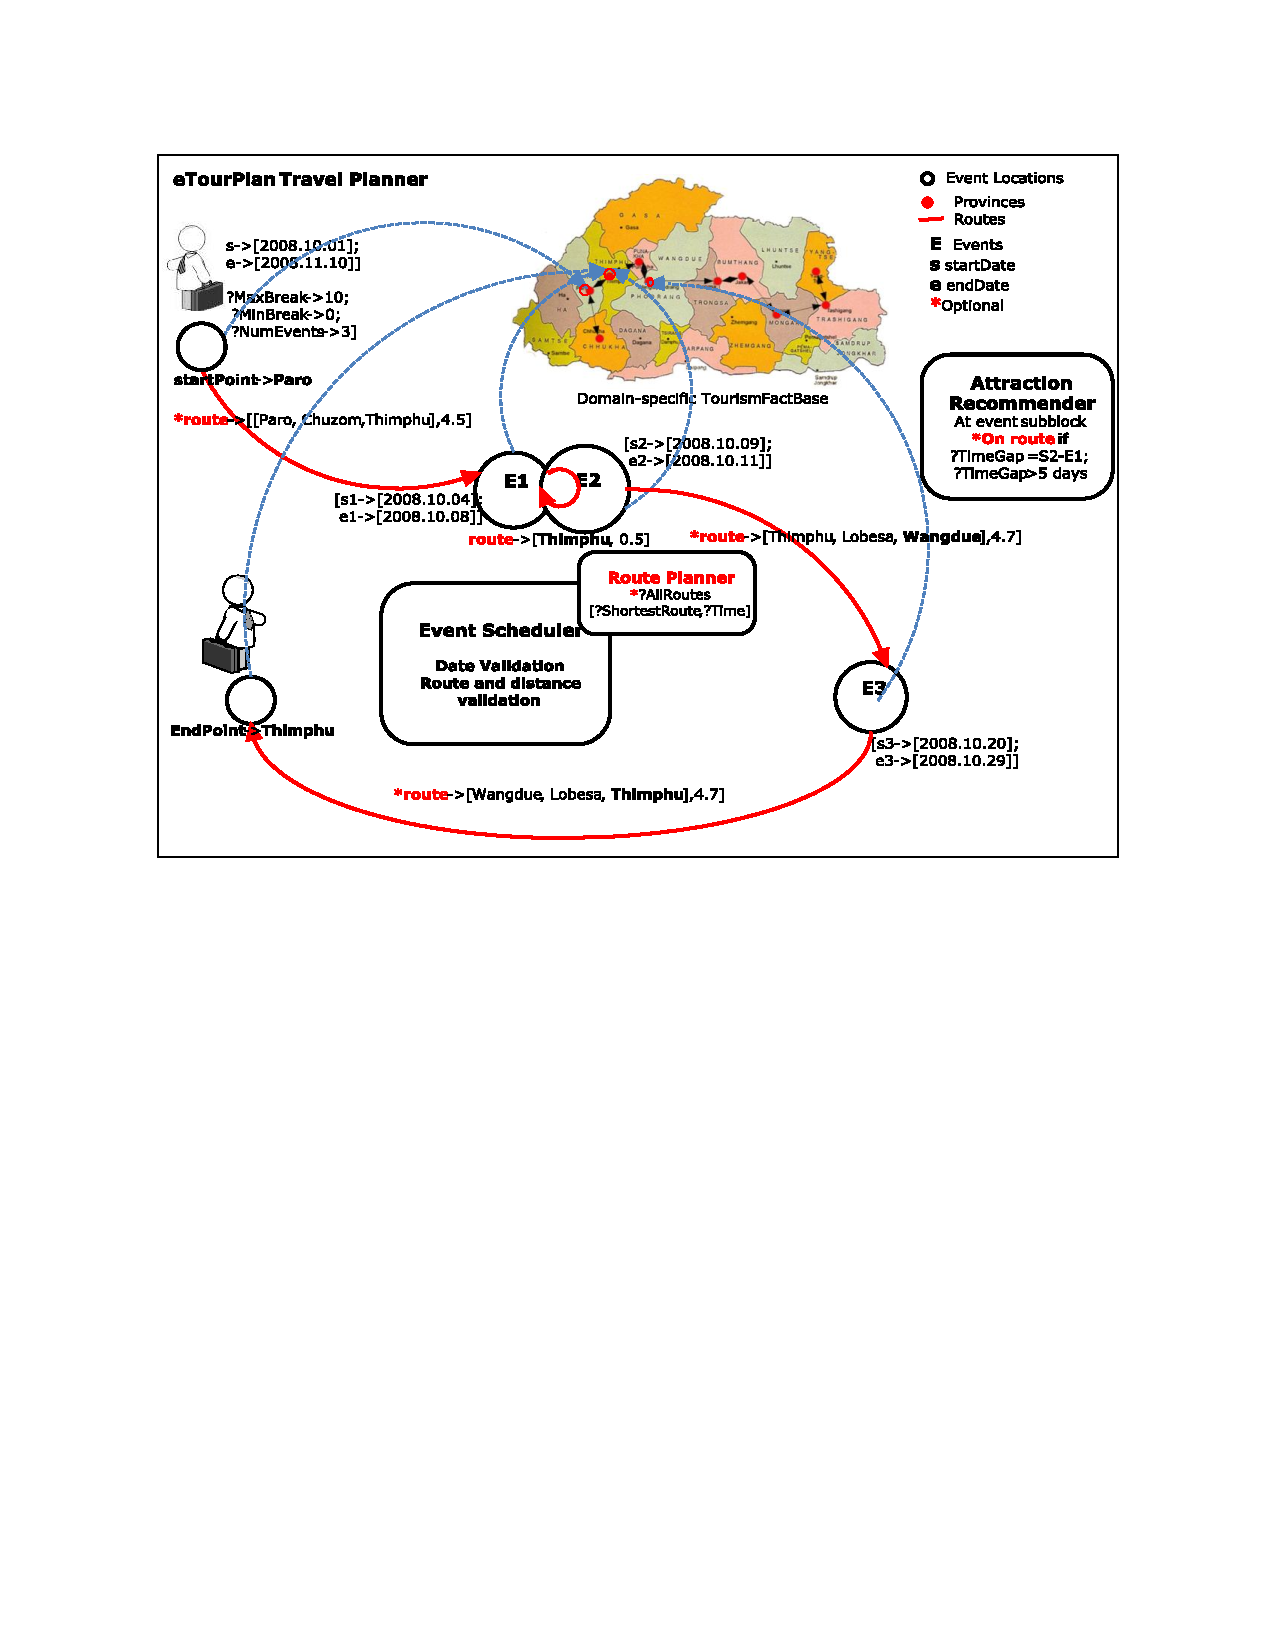
\includegraphics[width=11.5cm, height=7cm]{EventScheduling}
\caption{Travel Planning Scenario}
\end{figure}
}

\end{document}